\documentclass[twoside]{article} %用draft选项找到badbox的位置
%================================================
%     字体和页面布局
%================================================
%--------------------英文字体--------------------
\usepackage{fontspec}
%----英文字体第零套:用new roman------------------
%不用任何设置
%----英文字体第零1套:用new roman+dejavu----------
%\setmainfont[Ligatures=TeX]{DejaVu Serif}
%\setsansfont[Ligatures=TeX]{DejaVu Sans}
%\setmonofont[Ligatures=TeX]{DejaVu Sans Mono}
%----英文字体第零2套:用couriernew_libertine-----
%\setmonofont[Ligatures=TeX]{Courier New}
%\setmainfont[Ligatures=TeX]{Linux Libertine O}
%\setsansfont[Ligatures=TeX]{Linux Biolinum O}
%----英文字体第一套:衬线字体用new roman非衬线和等宽用Consolas---
%\setsansfont[Path="fonts/"]{PTSansNarrow.ttf}
%\setmonofont[Path="fonts/"]{PTSansNarrow.ttf}
%\setmonofont[Path="fonts/"]{YaHei.Consolas.ttf}
%----英文字体第二套:衬线字体用new roman非衬线和等宽用SourceCodePro---
%\setsansfont[Path="fonts/"]{SourceCodePro-Regular.otf}
%\setmonofont[Path="fonts/"]{SourceCodePro-Regular.otf}
%----英文字体第三套:全部用linuxLibertine--------
%\setmainfont{LinLibertine_R.otf}[
%Path="fonts/",
%BoldFont=LinLibertine_RB.otf,
%ItalicFont=LinLibertine_RI.otf,
%BoldItalicFont=LinLibertine_RBI.otf,
%SlantedFont = LinLibertine_aRL.ttf,
%BoldSlantedFont = LinLibertine_aBL.ttf,
%SmallCapsFont = LinLibertine_aS.ttf
%]
%\setsansfont{LinBiolinum_R.otf}[
%Path="fonts/",
%BoldFont=LinBiolinum_RB.otf,
%ItalicFont=LinBiolinum_RI.otf,
%BoldItalicFont=LinBiolinum_RBO.otf,
%]
%\setsansfont{LinLibertine_M.otf}[
%Path="fonts/",
%BoldFont=LinLibertine_MB.otf,
%ItalicFont=LinLibertine_MO.otf,
%BoldItalicFont=LinLibertine_MBO.otf,
%]
%--------------中文字体-----------------------
\usepackage[zihao=5]{ctex}
\usepackage{xeCJKfntef}
%--------中文字体第零套:采用windows字体-------
%\setCJKmainfont[BoldFont={SimHei},ItalicFont={KaiTi}]{NSimSun}
%\setCJKsansfont{SimHei}
%\setCJKmonofont{FangSong}
%\setCJKfamilyfont{zhsong}{NSimSun}
%\setCJKfamilyfont{zhhei}{SimHei}
%\setCJKfamilyfont{zhkai}{KaiTi}
%\setCJKfamilyfont{zhfs}{FangSong}
%\setCJKfamilyfont{zhli}{LiSu}
%\setCJKfamilyfont{zhyou}{YouYuan}
%----中文字体第一套:采用windows字体------------
%\setCJKmainfont[Path="fonts/",
%BoldFont={simhei.ttf},
%ItalicFont=simkai.ttf]{simsun.ttc}
%\setCJKsansfont[Path="fonts/"]{simhei.ttf}
%\setCJKmonofont[Path="fonts/"]{simfang.ttf}
%\setCJKfamilyfont{zhsong}[Path="fonts/"]{simsun.ttc}
%\setCJKfamilyfont{zhhei}[Path="fonts/"]{simhei.ttf}
%\setCJKfamilyfont{zhkai}[Path="fonts/"]{simkai.ttf}
%\setCJKfamilyfont{zhfs}[Path="fonts/"]{simfang.ttf}
%\setCJKfamilyfont{zhli}[Path="fonts/"]{simli.ttf}
%\setCJKfamilyfont{zhyou}[Path="fonts/"]{simyou.ttf}
%----中文字体第二套:采用adobe字体和思源字体----
%\setCJKmainfont[Path="fonts/",
%BoldFont={AdobeHeitiStd-Regular.otf},
%ItalicFont=AdobeKaitiStd-Regular.otf]{AdobeSongStd-Light.otf}
%\setCJKsansfont[Path="fonts/"]{AdobeHeitiStd-Regular.otf}
%\setCJKmonofont[Path="fonts/"]{AdobeFangsongStd-Regular.otf}
%\setCJKfamilyfont{zhsong}[Path="fonts/"]{AdobeSongStd-Light.otf}
%\setCJKfamilyfont{zhhei}[Path="fonts/"]{AdobeHeitiStd-Regular.otf}
%\setCJKfamilyfont{zhkai}[Path="fonts/"]{AdobeKaitiStd-Regular.otf}
%\setCJKfamilyfont{zhfs}[Path="fonts/"]{AdobeFangsongStd-Regular.otf}
%\setCJKfamilyfont{zhli}[Path="fonts/"]{NotoSansHans-Black.otf}
%\setCJKfamilyfont{zhyou}[Path="fonts/"]{NotoSansHans-Thin-Windows.otf}
%----------------中文字体命令定义-------------
%\renewcommand{\songti}{\CJKfamily{zhsong}} % 宋体
%\renewcommand{\heiti}{\CJKfamily{zhhei}}   % 黑体
%\renewcommand{\kaishu}{\CJKfamily{zhkai}}   % 楷书
%\newcommand*{\kaiti}{\CJKfamily{zhkai}}   % 楷书
%\renewcommand{\fangsong}{\CJKfamily{zhfs}} % 仿宋
%\renewcommand{\lishu}{\CJKfamily{zhli}}    % 隶书
%\renewcommand{\youyuan}{\CJKfamily{zhyou}} % 幼圆
%-----------------数学和其它字体-------------
\usepackage{bbding,pifont} %特殊字体,参考latexfriend
\usepackage{xltxtra} %用于输出tex的特殊文本格式,以及上下标的字符
\usepackage{mflogo,texnames}
%用于输出tex的特殊文本格式,texnames的说明文档没有找到
\usepackage{amsmath}
%使用宏包{美国数学协会数学},有个功能可以将章节和方程号联系起来。
\usepackage{amssymb} %使用宏包{美国数学协会符号}
%----------------页面布局、双栏----------------
\usepackage[a4paper,top=3cm, bottom=1.5cm, left=2.5cm, right=2.5cm]{geometry}
\renewcommand{\baselinestretch}{1.35}
\setlength{\headsep}{\baselineskip}%设置页面起始行与页眉间距
\usepackage{multicol}
\setlength{\columnsep}{5mm}
\setlength{\parskip}{2pt plus 2pt minus 2pt} %段落间距设置为0
\renewcommand{\abstractname}{} %摘要名不要
%\usepackage{balance}


%================================================
%     自定义信息和工具命令
%================================================
%-------------------辅助宏包---------------------
\usepackage{url}
\usepackage{lipsum}
\usepackage{xcolor}   %颜色
\usepackage{etoolbox} %latex编程辅助
\usepackage{ifthen}
%--------------标题,作者等信息输入--------------
\newcommand{\biaoti}[1]{\def\biaotiudf{#1}}
\def\fubiaotiudf{}
\newcommand{\fubiaoti}[1]{\def\fubiaotiudf{#1}}
%定义作者输入等处理命令
\DeclareListParser*{\forcsvlista}{;}
\def\schoolinput#1{\def\schoollistudf{}%将输入信息传入列表结构中
    \forcsvlista{\listadd\schoollistudf}{#1}}
\def\authorinput#1{\def\authorlistudf{}%
    \forcsvlista{\listadd\authorlistudf}{#1}}
\def\includinput#1{\def\includelistudf{}%
    \forcsvlista{\listadd\includelistudf}{#1}}

\newcounter{includeno}
\newcounter{authorno}
\newcounter{authorna}%all
\newcounter{schoolno}
\newcounter{schoolna}%all

\def\zuozhelist{%用于首页的作者信息
\setcounter{includeno}{0}%利用计数器将作者上标信息存入\listI等命令中
\renewcommand*{\do}[1]{\stepcounter{includeno}%
\expandafter\def\csname list\romannumeral\theincludeno\endcsname{##1}}
\dolistloop{\includelistudf}
\setcounter{authorno}{0}%利用计数器完成列表结构中的作者和上标信息结合
\renewcommand*{\do}[1]{\stepcounter{authorno}%
##1\textsuperscript{\csname list\romannumeral\theauthorno\endcsname}\hspace{1em}}%
\dolistloop{\authorlistudf}}

\def\zuozhelistb{%用于页眉的作者信息
\setcounter{authorna}{0}
\renewcommand*{\do}[1]{\stepcounter{authorna}}%计算总共有多少记录
\dolistloop{\authorlistudf}
\setcounter{authorno}{0}
\renewcommand*{\do}[1]{\stepcounter{authorno}
\ifnumless{\theauthorno}{\theauthorna}{##1\hspace*{1em}}{##1\listbreak}}
\dolistloop{\authorlistudf}}

\def\danweilistb{%用于首页的作者单位信息
\setcounter{schoolna}{0}%利用计数器确定列表结构中数据项总数
\setcounter{schoolno}{0}%利用计数器完成列表结构中的不同位置项的不同格式处理
\renewcommand*{\do}[1]{\stepcounter{schoolna}}%计算总共有多少记录
\dolistloop{\schoollistudf}
\renewcommand*{\do}[1]{\stepcounter{schoolno}%
\ifnumless{\theschoolno}{\theschoolna}{\theschoolno.##1\\}{\theschoolno.##1\listbreak}}%
\dolistloop{\schoollistudf}}

\newcommand{\zhaiyao}[1]{\def\zhaiyaoudf{#1}}
\newcommand{\guanjianci}[1]{\def\guanjianciudf{#1}}
\newcommand{\diyizuozhe}[1]{\def\diyizuozheudf{#1}}
\newcommand{\zuozhejianjie}[1]{\def\zuozhejianjieudf{#1}}

\newcommand{\qikanming}[1]{\def\qikanmingudf{#1}}
\newcommand{\nianfen}[1]{\def\nianfenudf{#1}}
\newcommand{\juanshu}[1]{\def\juanshuudf{#1}}
\newcommand{\qishu}[1]{\def\qishuudf{#1}}
\newcommand{\zongqishu}[1]{\def\zongqishuudf{#1}}

\newcommand{\zhongtu}[1]{\def\zhongtuudf{#1}}
\newcommand{\wenxianbiaozhi}[1]{\def\wenxianbiaozhiudf{#1}}
\newcommand{\wenzhangdoi}[1]{\def\wenzhangdoiudf{#1}}
\newcommand{\wenzhangbianhao}[1]{\def\wenzhangbianhaoudf{#1}}
%--------------首页通栏部分的样式---------------
\newenvironment*{lrindentlist}
  {\list{}{%
     \setlength{\leftmargin}{1cm}%
     \setlength{\rightmargin}{1cm}%
     \item\relax}}
  {\endlist}
\newcommand{\kongge}{\hspace*{1em}}
\def\temp{}
%\ifthenelse{\equal{\youwuudf}{\temp}}{true}{false}
\newcommand{\tonglan}{
\begin{center}
{\zihao{5}\heiti{Doi: }\wenzhangdoiudf\hfill
\heiti{文章编号: }\wenzhangbianhaoudf}\\
\vspace*{1.0cm}
{\heiti{\zihao{-2}{\biaotiudf}}}\\
{\vspace*{0.2cm}
%\ifx\fubiaotiudf\temp\vspace*{0.2cm}\else{\heiti\zihao{3}\fubiaotiudf}\\\fi
\ifthenelse{\equal{\fubiaotiudf}{\temp}}{\vspace*{0.2cm}}{\heiti\zihao{3}\fubiaotiudf\\}
%\ifdefempty{\fubiaotiudf}{\vspace*{0.2cm}}{\heiti\zihao{3}\fubiaotiudf\\}
\vspace*{0.2cm}}
{\kaishu\zihao{4}\zuozhelist}\\
{\vspace*{0.2cm}\kaishu\zihao{5}(\danweilistb)}
\end{center}
\begin{lrindentlist}
\zihao{5}\heiti{摘\kongge 要~~}\fangsong{\zhaiyaoudf}\par
\heiti{关键词~~}\fangsong{\guanjianciudf}\par
\heiti{中图分类号~~}\zhongtuudf\hfill \heiti{文献标志码~~}\wenxianbiaozhiudf\hspace*{4.5cm}
\end{lrindentlist}
\vspace{0.5cm}}

%================================================
%     目录/题注/页眉页脚/图表样式
%================================================
%--------------------图表题注--------------------
\usepackage{subfigure}
\usepackage{ccaption}
\captiondelim{~} %图序图题中间的间隔符号
\captionnamefont{\zihao{-5}\heiti} %图序样式
\captiontitlefont{\zihao{-5}\heiti} %图题样式
\captionwidth{0.8\linewidth} %标题宽度
\changecaptionwidth
%\captionstyle{<style>} can be used to alter this. Sensible values for
%style are: \centering, \raggedleft or \raggedright
\captionstyle{\centering}
%\precaption{\rule{\linewidth}{0.4pt}\par}
%\postcaption{\rule[0.5\baselineskip]{\linewidth}{0.4pt}}
\setlength{\belowcaptionskip}{0.1cm} %设置caption上下间距
\setlength{\abovecaptionskip}{0.1cm}
\setlength{\abovelegendskip}{0.1cm}  %设置legend上下间距
\setlength{\belowlegendskip}{0.1cm}
%注意用中文的图题时,用\\好像出错,而用\newline就没有问题
%采用\\到图列表中时需要用保护命令\protect如:

\newcommand{\listegcodename}{示~~ 例}
\newcommand{\egcodename}{示例}
\newfloatlist{egcode}{loc}{\listegcodename}{\egcodename}
\newfixedcaption{\codecaption}{egcode}
%目录命令
\renewcommand{\contentsname}{\Large\hfill 目~~录\hfill }
\renewcommand{\listfigurename}{\Large\hfill 插~~图\hfill }
\renewcommand{\listtablename}{\Large\hfill 表~~格\hfill }
%可以设置\cftbeforeZtitleskip,\cftafterZtitleskip长度,比如:
\setlength{\cftbeforeloctitleskip}{\baselineskip}
\setlength{\cftafterloctitleskip}{0.5\baselineskip}
%可以设置\cftZtitlefont字体样式比如
\renewcommand{\cftloctitlefont}{\hfill\Large\heiti}
\renewcommand{\cftafterloctitle}{\hfill}
\renewcommand{\cftegcodepresnum}{例}
\renewcommand{\cftegcodeaftersnum}{.}
\renewcommand{\cftegcodeaftersnumb}{~}
%\cftsetindents{egcode}{0em}{3em}
\setlength{\cftbeforeegcodeskip}{2mm}
\renewcommand{\cftegcodepagefont}{\bfseries}

%浮动体外使用标题,使用\tabcaptionfix命令产生在浮动体外
%与table中默认的caption一致的标题效果
\newfixedcaption{\tabcaption}{table}
\newfixedcaption{\figcaption}{figure}
%\newfixedcaption{\tabcaptionfix}{table}

%双语标题
%\bitwonumcaption[label]{short-1}{long-1}{NAME}{short-2}{long-2}
%其中,label为标签,替代普通的\label
%short-1,第一种语言的短标题
%long-1,第一种语言的长标题
%name,第二中语言的图序名称,如:英语的fig,中文的图
%short-2,第二种语言的短标题
%\bionenumcaption,与\bitwonumcaption类似,差别在于第二种语言在目录中不列序号
%\bicaption[label]{short-1}{long-1}{NAME}{long-2},
%也是类似,差别在于第二中语言不列入目录中
%\midbicaption,类似于precaption和postcaption,双语标题,其本质是两次调用caption
%使用\midbicaption命令就是在调用第二次caption前重设precaption和postcaption
%比如\precaption{\rule{\linewidth}{0.4pt}\par}\postcaption{}
%\midbicaption{\precaption{}\postcaption{\rule{\linewidth}{0.4pt}}}

%续表的双语标题使用命令:
%\bicontcaption{long-1}{NAME}{long-2}

%注意ccaption与longtable一起使用,longtable需要在ccaption前调用
%且双语的标题略有不同,需要特定的命令如下:
%\longbitwonumcaption
%\longbionenumcaption
%\longbicaption
%\midbicaption

%关于子图的标题,利用宏包subfigure,具体参见说明文档2.5节
%关于浮动体放文章最后的情况,利用宏包endfloat,具体参见说明文档2.6节

%----------------------插入图片--------------------
\usepackage{graphicx}
%\usepackage{graphics}
\DeclareGraphicsExtensions{.eps,.mps,.pdf,.jpg,.png}
\DeclareGraphicsRule{*}{eps}{*}{} %%声明不是eps结尾的图片都当成eps处理
\graphicspath{{graph/}{img/}{./exampleandimage/}} %设置图片放置的位置
\def\figwd{0.6}%全局设置插图宽度与textwidth之比

%=====================tikz绘图===============================================
\usepackage{pgf,tikz} %做tikz图所用宏包
\usepackage{mathrsfs}
%\usetikzlibrary{arrows}
%\pagestyle{empty}
\newcommand{\degre}{\ensuremath{^\circ}}

%\usepackage{pgf}
%\usepackage{pgfmath}
%\usepackage{tikz}
\usepgfmodule{shapes}
\usetikzlibrary{arrows,decorations.pathmorphing,backgrounds,positioning,fit,petri}
\usetikzlibrary{math,mindmap,shapes.geometric,calc,intersections,through}
\usetikzlibrary{knots}

\colorlet{examplefill}{yellow!80!black}
\definecolor{graphicbackground}{rgb}{0.96,0.96,0.8}
\definecolor{codebackground}{rgb}{0.9,0.9,1}
\definecolor{lightblue}{RGB}{199,232,250}
\definecolor{darkblue}{RGB}{59,134,215}

%\tikzstyle{startstop}=[rectangle,rounded corners,minimum width=2cm,minimum height=1cm,fill=red!30,text centered]
%\tikzstyle{process}=[rectangle,rounded corners,minimum width=2cm,minimum height=1cm,fill=orange!30,text centered]
%\tikzstyle{decision}=[diamond,minimum width=2cm,minimum height=1cm,fill=green!30,text centered]
%\tikzstyle{io}=[trapezium,trapezium left angle=70,trapezium right angle=110,minimum width=2cm,minimum height=1cm,fill=blue!30,text centered]
%\tikzstyle{arrowseta}=[thick,->,>=stealth]
%\tikzstyle{arrowsetb}=[thick,<-,>=stealth]

\newenvironment{insertfigure}[2]%
{\begingroup\def\figcaptioninfo{#1}\def\figlabelinfo{#2}\centering}%
{\figcaption{\figcaptioninfo}\label{\figlabelinfo}\par\endgroup}

%-------------------表格相关--------------------
\usepackage{multirow} %for excel2latex
\usepackage{booktabs} %for excel2latex
\usepackage{array}
\usepackage{tabularx}
%\usepackage{longtable} %注意longtable无法在multicol中使用
\usepackage{supertabular} %使用supertabular来实现可以跨页的表格

\newenvironment{inserttable}[2]%
{\begingroup\tabcaption{#1}\label{#2}\par\noindent\centering}%
{\par\endgroup}

%--------------标题样式和页眉页脚定义-------------
\usepackage[pagestyles]{titlesec}
%注意titlesec带pagestyles选项之后与fancyhdr宏包有冲突,所以使用要注意
\titleformat{\section}{\zihao{4}\heiti}{\thesection}{1em}{}
\titlespacing*{\section}{0pt}{0.5\baselineskip}{0.5\baselineskip}[0pt]
\titleformat{\subsection}{\zihao{5}\heiti}{\thesubsection}{1em}{}
\titlespacing*{\subsection}{0pt}{0pt}{0pt}[0pt]
%\titleformat{\subsubsection}{\zihao{5}\songti}{\thesubsubsection}{1em}{}
\titleformat{\subsubsection}{\zihao{5}\heiti}{\thesubsubsection}{1em}{}
\titlespacing*{\subsubsection}{0pt}{0pt}{0pt}[0pt]
%设置页面页脚线存在bug不能直接设置\setheadrule{~pt}默认的宽度会冲掉它
%所以使用下面的两句重定义命令进行修改
\renewcommand\headrule{\setheadrule{1pt}}
\renewcommand\footrule{\setfootrule{0pt}}

\newpagestyle{main}{ %%内容奇数页左,偶数页右
\sethead[{\zihao{-5}~\thepage~}]%偶数页左
[{\zihao{-5}~\qikanmingudf}]%偶数页中
[{\zihao{-5}\nianfenudf 年第\juanshuudf 卷}]%偶数页右
{{\zihao{-5}~第\qishuudf 期}\hfil}%奇数页左
{{\zihao{-5}\zuozhelistb :~\biaotiudf ~\fubiaotiudf}}%奇数页中
{{\zihao{-5}~\thepage~}}%奇数页右
\setfoot{}{}{}%
\headrule%
\footrule}%

\newpagestyle{firstpageps}{ %%内容奇数页左,偶数页右
\sethead[{\zihao{-5}~\thepage~~\qikanmingudf}]%偶数页左
[]%偶数页中
[\raisebox{0.0\baselineskip}{\parbox{7cm}{\raggedleft\zihao{-5}\nianfenudf 年第\juanshuudf 卷第\qishuudf 期(总第\zongqishuudf 期)}}]%偶数页右
{{\zihao{-5}~\qikanmingudf}}%奇数页左
{}%奇数页中
{\raisebox{0.0\baselineskip}{\parbox{7cm}{\raggedleft\zihao{-5}\nianfenudf 年第\juanshuudf 卷第\qishuudf 期(总第\zongqishuudf 期)~~~~\thepage~}}}%奇数页右
\setfoot{%\ ~
%\vspace{0.5cm}
\rule[2\baselineskip]{0.3\linewidth}{0.4pt}
\raisebox{\baselineskip}{\hspace*{-0.3\linewidth}\parbox{\linewidth}{\renewcommand{\baselinestretch}{1.0}%
\large\normalsize\raggedright{\heiti\zihao{6}{\diyizuozheudf}}%
{\kaishu\zihao{6}\zuozhejianjieudf}}}
}{}{}%
\headrule}%
%\footrule}%


%================================================
%        超链接,参考文献
%================================================
\usepackage[CJKbookmarks,%
colorlinks=true,%
bookmarksnumbered=true,%
pdfstartview=FitH,%
linkcolor=magenta,%
anchorcolor=magenta,%
citecolor=magenta]{hyperref}   %书签功能,选项去掉链接红色方框,
%linkcolor=black,linkcolor=green,blue,red,cyan, magenta,
%yellow, black, gray,white, darkgray, lightgray, brown,
%lime, olive, orange, red,purple, teal, violet.
%下面这两句保证多篇文章一起排时的超链接正确性
\newcounter{Hsection}
\preto\section{\stepcounter{Hsection}}
\usepackage{titleref} %标题引用
%-------------------参考文献---------------------
%\usepackage[backend=bibtex8,sorting=none,citestyle=authoryear,bibstyle=alphabetic]{biblatex}
%采用分章的参考文献的快捷方法
\usepackage[backend=biber,backref=true,%
style=gb7714-2015]{biblatex}%biber
\renewcommand{\bibfont}{\zihao{-5}\songti}
\setlength{\bibitemsep}{2pt}
\defbibheading{bibliography}[\bibname]{%
	\section*{#1}}%
%	\markboth{#1}{#1}}
%注意在实际使用中用titsec宏包的页眉页脚也有点问题,一旦给出markboth就会出现问题
%这里因为bibliography给出了markboth所以出错。因此重定义bibliography以消除问题
%重定义命令中去掉了markboth那一句命令。
%常用样式
%style=trad-plain
%style=trad-unsrt
%style=trad-alpha
%style=trad-abbrv
%style=musuos
%style=nature
%style=nejm  %New England Journal of Medicine
%style=phys  %follows the guidelines of the aip and aps
%bibstyle=publist
%style=science  %follows the guidelines of the journal Science

%style=ieee % follows the guidelines of the ieee.
%style=ieee-alphabetic
%bibstyle=manuscripts,otheroption
%style=chem-acs %American Chemistry Society journals.
%style=chem-angew %Angewandte Chemie Chemistry – A European Journal.
%style=chem-biochem %Biochemistry and a small number of other American Chemistry Society journals.
%style=chem-rsc  %Royal Society of Chemistry journals.
%style=authortitle-dw
%style=footnote-dw



%================================================
%    代码呈现环境;listings宏包
%================================================
\usepackage{listings}
\lstnewenvironment{texlist}%
{\lstset{% general command to set parameter(s)
%name=#1,
%label=#2,
%caption=\lstname,
linewidth=\linewidth,
breaklines=true,
%showspaces=true,
extendedchars=false,
columns=fullflexible,%flexible,
frame=none,
fontadjust=true,
language=[LaTeX]TeX,
%backgroundcolor=\color{yellow}, %背景颜色
%numbers=left,
%numberstyle=\tiny\color{red},
basicstyle=\scriptsize, % print whole listing small
keywordstyle=\color{blue}\bfseries,%\underbar,
% underlined bold black keywords
identifierstyle=, % nothing happens
commentstyle=\color{green!50!black}, % white comments
stringstyle=\ttfamily, % typewriter type for strings
showstringspaces=false}% no special string spaces
}
{}

\lstnewenvironment{fortranlist}%
{\lstset{% general command to set parameter(s)
%name=#1,
%label=#2,
%caption=\lstname,
linewidth=\linewidth,
breaklines=true,
%showspaces=true,
extendedchars=false,
columns=fullflexible,%flexible,
frame=none,
fontadjust=true,
language=[08]Fortran,
%backgroundcolor=\color{yellow}, %背景颜色
%numbers=left,
%numberstyle=\tiny\color{red},
basicstyle=\scriptsize, % print whole listing small
keywordstyle=\color{blue}\bfseries,%\underbar,
% underlined bold black keywords
identifierstyle=, % nothing happens
commentstyle=\color{green!50!black}, % white comments
stringstyle=\ttfamily, % typewriter type for strings
showstringspaces=false}
} % no special string spaces}
{}

\lstnewenvironment{mathlist}%
{\lstset{% general command to set parameter(s)
%name=#1,
%label=#2,
%caption=\lstname,
linewidth=\linewidth,
breaklines=true,
%showspaces=true,
extendedchars=false,
columns=fullflexible,%flexible,
frame=none,
fontadjust=true,
language=[5.2]Mathematica,
%backgroundcolor=\color{yellow}, %背景颜色
%numbers=left,
%numberstyle=\tiny\color{red},
basicstyle=\scriptsize, % print whole listing small
keywordstyle=\color{blue}\bfseries,%\underbar,
% underlined bold black keywords
identifierstyle=, % nothing happens
commentstyle=\color{green!50!black}, % white comments
stringstyle=\ttfamily, % typewriter type for strings
showstringspaces=false}
} % no special string spaces}
{}

\lstnewenvironment{codetex}[2]%
{\begin{center}\end{center}\centering\setlength{\abovecaptionskip}{1mm}\setlength{\belowcaptionskip}{1mm}%
\vspace{-2\baselineskip}
\codecaption{#1}\label{#2}%\nopagebreak
\vspace{-1.0\baselineskip}
\lstset{%general command to set parameter(s)
%name=#1,
%label=#2,
%caption=\lstname,
linewidth=\linewidth,
breaklines=true,
%showspaces=true,
extendedchars=false,
columns=fullflexible,%flexible,
frame=tb,
%frame=none,
fontadjust=true,
language=[LaTeX]TeX,
%backgroundcolor=\color{yellow}, %背景颜色
backgroundcolor=\color{codebackground},
fillcolor=\color{codebackground},
rulecolor=\color{green!50!black},
numbers=left,
numberstyle=\tiny\color{red},
basicstyle=\footnotesize, % print whole listing small,footnotesize
keywordstyle=\color{blue}\bfseries,%\underbar,
% underlined bold black keywords
identifierstyle=, % nothing happens
commentstyle=\color{green!50!black}, % white comments
stringstyle=\ttfamily, % typewriter type for strings
showstringspaces=false}% no special string spaces
%\renewcommand{\baselinestretch}{0.95}
\ifodd\thepage{
\begin{tikzpicture}[overlay,remember picture]
\node[fill=yellow!50,inner sep=1pt] at ($(-0.5\linewidth,-2mm)-(4mm,0mm)$) {\tiny{代码}};
\end{tikzpicture}}
\else{
\begin{tikzpicture}[overlay,remember picture]
\node[fill=yellow!50,inner sep=1pt] at ($(0.5\linewidth,-2mm)+(4mm,0mm)$) {\tiny{代码}};
\end{tikzpicture}}
\fi
}{}



\usepackage[inline]{enumitem} %重设list环境
\setlist[itemize]{label=\color{blue}$\blacktriangleright$,topsep=2pt,partopsep=0pt,parsep=0pt,%
itemsep=0pt,leftmargin=2em}%label=$\triangleright$
%\setlist[itemize]{topsep=2pt,partopsep=0pt,parsep=0pt,%
%itemsep=0pt,leftmargin=4em}%label=$\triangleright$
\setlist[enumerate]{topsep=2pt,partopsep=0pt,parsep=0pt,%
itemsep=0pt,leftmargin=4em}%label=$\triangleright$
\setlist[description]{topsep=5pt,partopsep=0pt,parsep=0pt,%
itemsep=0pt,leftmargin=2cm,rightmargin=0cm,labelwidth=2cm}

\newcommand{\qd}[1]{%定义qd为强调命令
{\bfseries\color{violet}#1}}
%orange,brown,purple,teal,violet,olive,cyan


%%----------------------------------------------------------------------
%%                  参考文献库添加
%%----------------------------------------------------------------------
\addbibresource[location=local]{./exampleandimage/example.bib}
%论文1的参考文献的bib文件

%%----------------------------------------------------------------------
%%                  正文
\begin{document}
%%----------------------------------------------------------------------

%----------------------------------------------------------------------
%                  第一篇论文-填写基本信息
%----------------------------------------------------------------------
\qikanming{\LaTeX 爱好者}                       %期刊名,journal name
\nianfen{2016}                                  %年份,year
\juanshu{1}                                    %卷数,volume
\qishu{1}                                       %期数,number
\zongqishu{99}                                  %总期数,

\wenzhangdoi{10.11729/tex-lover}                   %doi号
\wenzhangbianhao{1672-9897(2016)01-0000-00}   %文章编号
\zhongtu{(V211.751)}                          %中图分类号
\wenxianbiaozhi{A}                              %文献标志码

\biaoti{\LaTeX 文档中文参考文献的biblatex解决方案}                     %标题,title
\fubiaoti{}                               %副标题,subtitle

\authorinput{胡振震} %作者间用英文分号隔开
\schoolinput{~LEETC~~CHINA~~100000~}                        %单位间用英文分号隔开
\includinput{1}              %各作者所属单位用英文分号隔开,
                                     %一位作者的多个所属单位用英文逗号隔开

                                                %摘要,abstract
\zhaiyao{针对\LaTeX 文档的中文参考文献问题,对其需求展开分析,提出利用biblatex宏包的解决思路,并针对性地给出了各项需求的解决方案(包括示例代码),为\LaTeX 文档参考文献生成提供便利。}

                                                %关键词,keywords
                                                %多个关键词用\kongge隔开
\guanjianci{\LaTeX \kongge 参考文献 \kongge biblatex}
                                                %use \kongge as separation

                                          %收稿等时间,第一/通信作者简介,
\def\versionnumber{v1.0}    %版本和修改时间信息
\def\versiondate{2016-12-07}
\diyizuozhe{The files have version number \versionnumber, last revised \versiondate.\\ 第一作者简介:}
                                          %introduction of corresponding author
\zuozhejianjie{HU ZHENZHEN,A \LaTeX ~LOVER,Email: hzzmail@163.com。}


%----------------------------------------------------------------------
%                  第一篇论文-正文内容
\tonglan
\thispagestyle{firstpageps}
\pagestyle{main}
\setcounter{section}{-1}
\enlargethispage{-1.0\baselineskip}
%\begin{refsection}
%\begin{multicols}{2}
%\makeatletter
%\let\mcnewpage=\newpage
%\newcommand{\TrickSupertabularIntoMulticols}{%
%  \renewcommand\newpage{%
%    \if@firstcolumn
%      \hrule width.918\linewidth height0pt
%       \columnbreak
%    \else
%      \mcnewpage
%    \fi
%  }%
%}
%\makeatother 
%----------------------------------------------------------------------
\section{引言}

参考文献是科技文档写作中的重要组成部分。在写作中常碰到这样的问题包括:怎么在文档合适位置插入满足格式要求的参考文献引用?怎么生成满足格式要求的参考文献表?怎么采用不同的宏包实现一些特殊的功能如分章文献?等等。这些问题尽管不会成为困扰,但的确会牵扯写作者不少精力。为帮助\LaTeX 文档作者能够更快更简便的进行参考文献生成,有必要对参考文献问题的解决方案进行梳理和总结,以便其能够随时参考、移植和应用。一般需求的参考文献生成其实并不困难,采用传统的\LaTeX 的方法就可以满足,该方法的具体实践可以参考刘海洋\cite{刘海洋2013--}或者胡伟\cite{胡伟2011--}的专著。但是如果需要实现一些复杂的非常规的功能,就可能需要应用一些其他宏包,比如chapterbib,natbib等,这样问题就变得复杂起来。事实上随着biblatex宏包的完善,利用它可以满足对于参考文献的绝大多数功能需求。如果利用一个宏包就能完成以前多个宏包才能实现的功能,那么问题实际上就简化了,这正是用户所期待的。利用biblatex宏包“简单化、便利化”地满足\LaTeX 文档写作中的各种中文参考文献需求也正是本文写作的初衷所在。

关于biblatex宏包的详细介绍可以参考其手册\cite{Lehman2015}和biblatex-gb7714-2015样式包的说明文档\cite{胡振震2016}。需要注意的是本文所有的示例和说明都基于texlive平台,2015或者2016都可以,文档均采用UTF-8编码,编译使用xelatex,texlive的安装可以参考texlive安装手册\cite{Berry2016--}以及ctex论坛或latex开源小屋分享的各种方法。

\section{需求分析}
\LaTeX 中文写作对于参考文献一般会有哪些需求?最直接的,我们会想到文章投稿时的参考文献格式要求,比如:参考文献标题的字体字号前后间距段落格式;参考文献内容的字体字号;各条目的间距;条目的内容格式如文献标识符、标点等;双语参考文献;上标、带年份、带页码等标注要求等等。在书籍之类的文档排版中有时也会遇到比如:分章参考文献表;文后参考文献总表;参考文献的目录链接;脚注中引用参考文献;脚注中直接显示参考文献;在合适位置按需插入文献表等等。还有一些比如文献的排序;PDF文档中标注和文献条目的正反超链接等。总结起来可能包括如下11条需求(注意这里所列的不是全的,一些未遇到过的新问题并不在其中,只能以后完善,也希望大家帮助一起完善),这里根据本文作者的理解,按照重要程度列出:
\begin{enumerate}
  \item 参考文献表基本生成方法-数据源文件准备(手动、利用winedt、利用texstudio 、Jabref、\LaTeX 文档生成)
  \item 参考文献表基本生成方法-文档的组成(基本结构、宏包加载、样式包加载、文献引用、文献表打印)
  \item 参考文献表基本生成方法-文档的编译(手动、利用winedt、利用texstudio、脚本)
  \item 书后参考文献和分章参考文献
  \item 参考文献标题格式(重定义heading,利用titlesec)
  \item 参考文献内容格式(重定义内容命令)
  \item 参考文献著录样式(顺序制、作者年制、域、位置、标点、排序)
  \item 参考文献标注样式(页码、年份)
  \item 多语言文献
  \item 脚注题注小页环境中的引用
  \item 脚注旁注中的文献表
  \item 文献表的分类筛选打印
  \item beamer类中的参考文献
\end{enumerate}

\section{解决方案}
本节直接针对上一节提出的需求,逐条进行处理。方案主要应用于一般文档类(book,report,article),beamer类的问题专门放到最后一条中介绍。
\subsection{数据源文件准备}
\LaTeX 文档中生成参考文献除了利用thebibliography环境手工输入参考文献条目信息这一简单方式外,其它方式都需要一个参考文献数据源文件即bib文件。在这一文件内保存各类型参考文献的信息,每一条参考文献信息都是一个bibtex item(bibtex项),其基本格式如下:
\begin{codetex}{参考文献信息基本格式}{fmt:bibtex}
@ARTICLE{entrykey,
  author =       {},
  title =        {},
  journal =      {},
  year =         {},
  volume =       {},
  number =       {},
  pages =        {},
  month =        {},
}
\end{codetex}

其中\@后面紧跟着条目的类型比如article(期刊文章),book(专著)等,编组符号\{后紧跟的是该条参考文献信息的bibtex key即引用关键词,在cite引用命令中用该词来表示对此文献的引用。逗号后面跟着的是参考文献的所有各个域的信息,比如作者域,题名域等等,参考文献信息放在各个域名等号后面的编组内,一些域的录入比如author域的英文名录入是有特殊格式要求的,具体可以参考文献\cite{胡振震2016}中关于域信息录入的说明。参考文献源文件只是一个文本文件,只是其内容需要遵守bibtex格式,所以其生成可以有多种方式。

\subsubsection{手动文本文件生成}

利用文本编辑器比如notepad++等,生成或者编辑bib源文件是一种很简单的方式,直接新建bib文件,用notepad++打开,填入需要的参考文献信息,保存就可以得到一个bib源文件,如图\ref{bib:texteditor}所示。notepad++,notepad2等文本编辑器均可在其官网下载到。

\begin{figure}[!htb]
  \centering
  \includegraphics[width=\figwd\textwidth]{bib-text-editor.jpg}
  \caption{文本编辑器生成bib文件}\label{bib:texteditor}
\end{figure}

\subsubsection{利用winedt生成}
在windows下常用winedt编辑latex文档,所以用其生成bib文件也是一种不错的方式,特别是它提供了各种条目类型的信息模板(图\ref{bib:winedt})。winedt可以在其官网(\url{http://www.winedt.com/})下载到,非注册版本不影响功能使用。

\begin{figure}[!htb]
  \centering
  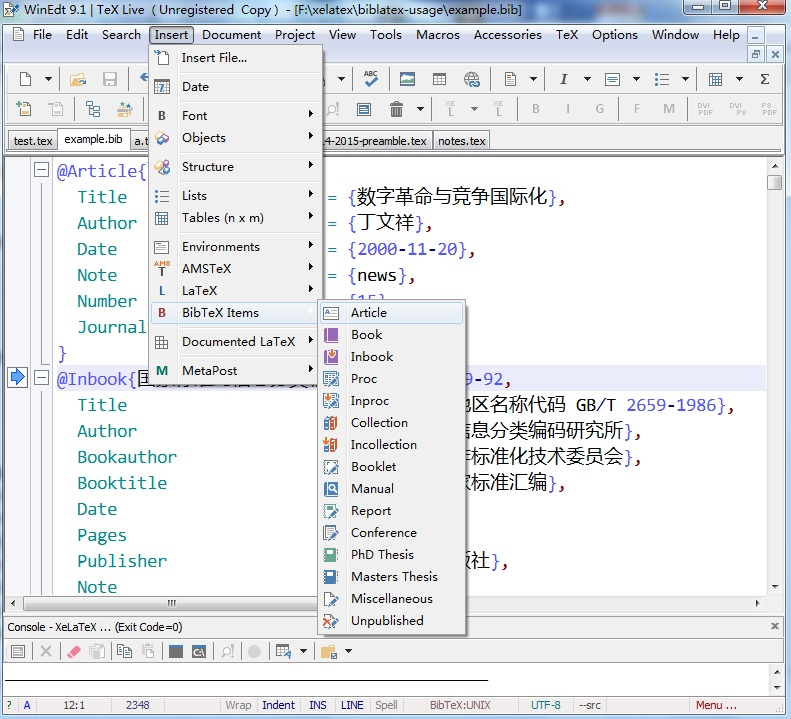
\includegraphics[width=\figwd\textwidth]{bib-winedt.jpg}
  \caption{winedt生成bib文件}\label{bib:winedt}
\end{figure}

\subsubsection{利用texstudio生成}
texstudio软件可以在多平台使用,linux下因为没有winedt所以比较常用,用其生成bib文件也很方便,它也提供各种条目类型的信息模板(图\ref{bib:texstudio})。texstudio软件下载地址\url{https://sourceforge.net/projects/texstudio/?source=navbar}。

\begin{figure}[!htb]
  \centering
  \includegraphics[width=\figwd\textwidth]{bib-texstudio.jpg}
  \caption{texstudio生成bib文件}\label{bib:texstudio}
\end{figure}

\subsubsection{利用Jabref软件生成}
利用Jabref软件是最重要的一种方式,因为它也是一个较强的参考文献管理工具。新建一个数据库就是新建一个bib文件(图\ref{bib:jabref-a}),新建一个记录就是加入一条参考文献信息(图\ref{bib:jabref-b}),参考文献的信息的录入也是可视化输入栏形式(图\ref{bib:jabref-c})。jabref软件可在官网(\url{http://www.jabref.org/})下载。

\begin{figure}[!htb]
  \centering
  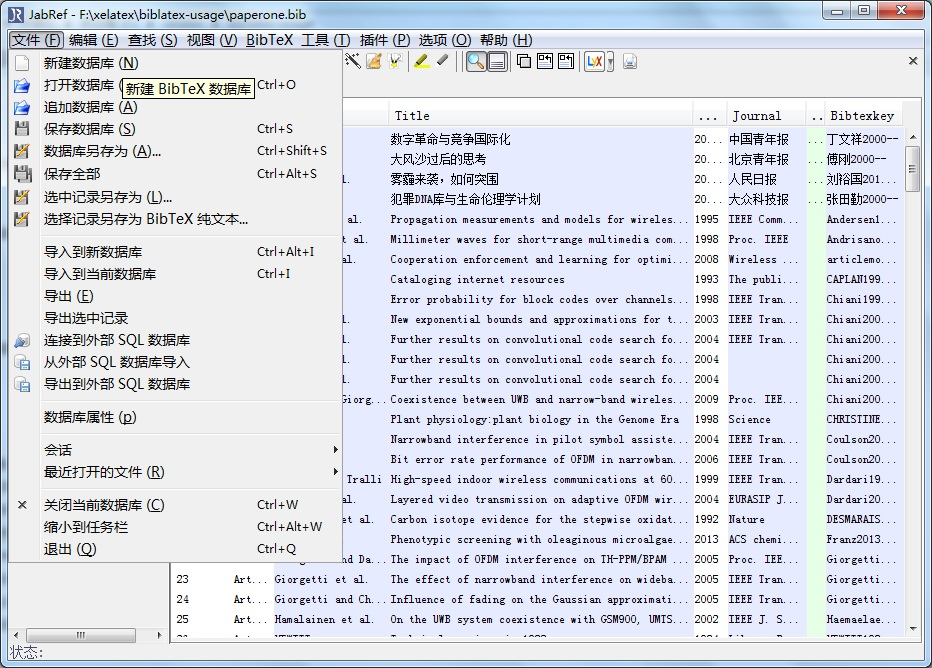
\includegraphics[width=\figwd\textwidth]{bib-jabref-a.jpg}
  \caption{Jabref软件生成bib文件}\label{bib:jabref-a}
\end{figure}

\begin{figure}[!htb]
  \centering
  \includegraphics[width=\figwd\textwidth]{bib-jabref-b.jpg}
  \caption{Jabref软件增加参考文献条目}\label{bib:jabref-b}
\end{figure}

\begin{figure}[!htb]
  \centering
  \includegraphics[width=\figwd\textwidth]{bib-jabref-c.jpg}
  \caption{Jabref软件录入参考文献信息}\label{bib:jabref-c}
\end{figure}

\subsubsection{随\LaTeX 文档生成}
\LaTeX 提供了filecontents环境允许在\LaTeX 文档编译的时候自动将信息写入文件中,自然这也可以用来生成bib文件。比如在导言区加入如下代码,可以生成一个example.bib源文件。
\begin{codetex}{利用filecontents环境随latex文档生成bib}{bib:genwithlatex}
\usepackage{filecontents}
\begin{filecontents}{example.bib}
@Article{傅刚2000--,
  Title                    = {大风沙过后的思考},
  Author                   = {傅刚 and 赵承 and 李佳路},
  Note                     = {news},
  Number                   = {14},
  Url                      = {http://www.bjyouth.com.cn/Bqb/20000412/GB/4216%5ED0412B1401.htm},
  Urldate                  = {2005-07-12},
  Date                     = {2000-04-12},
  Journaltitle             = {北京青年报}
}
@Book{顾炎武1982--,
  Title                    = {昌平山水记},
  Author                   = {顾炎武},
  Publisher                = {北京古籍出版社},
  Year                     = {1982},
  Location                 = {北京},
  Titleaddon               = {东京考古录}
}
\end{filecontents}
\end{codetex}

\subsubsection{获取标准bib文件}
上述给出的方法都是手动编写bib文件的方法,事实上这些手工编写方法还是比较繁琐的。那么是否有其它方法可以获取bib文件或其内容避免自己手工编写呢?答案是有的,latexstudio上共分享了几篇文章\cite{北京交通大学研究生公众号2016--}\cite{olref2016--}\cite{文献助手2016--}。总结起来主要有几个渠道:
\begin{enumerate}
  \item Google 学术: 检索文献 >> Cite(引用) >> BibTeX >> 复制粘贴到 mybibtex.bib 文件
  \item CNKI,(以 firefox 为例): (确保安装 Zotero 的 firefox 扩展 >>) CNKI 检索文献 >> 点击一下 url 输入框末尾的文件夹图标 >> 选中要导出的文献 >> 导出为 BibTeX 引用格式 >> 复制粘贴导出的 BibTeX 文献到 mybibtex.bib 文件。
  \item 必应学术(必应 学术 – 学无止境,术有乾坤)、百度学术(百度学术 – 保持学习的态度)类似于google学术。
  \item 学术性期刊的官网都是可以直接获取bib文件的,比如IEEE,Springer,Elsevier等等
  \item 使用文献助手工具,地址:\url{http://cite.latexstudio.net}
\end{enumerate}
熟练使用这些方法,应该可以有效提高工作效率。

\subsection{文档的组成}
\LaTeX 文档源文件是由具有某一结构和模式的代码所构成,参考文献的生成自然也遵守这样的结构和模式。

\subsubsection{文档源文件基本结构}
\LaTeX 文档源文件的代码基本结构由导言区正文区构成,导言区处于documentclass命令与begin\{document\}命令之间,而正文区处于begin\{document\}命令和end\{document\}命令之间。宏包在导言区加载,具体文档内容在正文区编辑。
\begin{codetex}{文档源文件的代码基本结构}{code:doc:structrue}
\documentclass{article}%文档类

%导言区:
%ctex中文设置
\usepackage{ctex}
%定义版面
\usepackage[paperwidth=210mm,paperheight=290mm,left=20mm,right=20mm,top=25mm, bottom=15mm]{geometry}
%书签功能,选项去掉链接红色方框
\usepackage[colorlinks=true,pdfstartview=FitH,linkcolor=blue,anchorcolor=violet,citecolor=magenta]{hyperref}

\begin{document}%正文区开始
正文内容
\end{document}
\end{codetex}

\subsubsection{biblatex宏包、参考文献数据源和样式的加载}
biblatex宏包和参考文献数据源都在导言区加载(例\ref{code:pkg:load}),宏包加载命令为usepackage,数据源加载命令为addbibresource。参考文献样式作为biblatex宏包的可选参数加载,即用bibstyle选项设置著录样式,用citestyle选项设置标注样式,当两者使用同名样式时,可以用一个选项style表示,例\ref{code:pkg:load}中bibstyle和citestyle都选择使用gb7714-2015样式。为利用biblatex实现复杂功能,后端backend采用biber而不用bibtex(如果backend为bibtex8是利用bibtex和aux文件进行类似于\LaTeX 传统方法的编译,而使用backend为biber则是利用生成的bcf文件进行编译)。参考文献样式还可以使用biblatex宏包提供的标准样式(标准样式详见biblatex手册Standard Styles一节),或者使用其它作者提供的定制样式,比如nature,science等。
\begin{codetex}{biblatex宏包、数据源和样式的加载}{code:pkg:load}
%biblatex宏包加载
%其中后端backend使用biber
%引用样式citestyle,著录样式bibstyle都采用gb7714-2015样式
\usepackage[backend=biber,bibstyle=gb7714-2015,%nature,%
citestyle=gb7714-2015%,backref=true%
]{biblatex}

%参考文献数据源加载
\addbibresource[location=local]{example.bib}
\end{codetex}

值得注意的是:参考文献数据库源文件即bib文件可以是本地的,也可以是网络上的(具体参考biblatex手册Bibliography Commands一节中关于addbibresource命令的说明)。本地的数据源可以指定绝对路径或者相对路径,注意其中目录层级之间的间隔符用/而不是\textbackslash ,windows下默认复制的间隔符是\textbackslash ,需要将其改为/。添加数据源的例子参考例\ref{ref:addresource}。

\begin{codetex}{添加参考文献数据源的两种方式}{ref:addresource}
\addbibresource{bibfile1.bib} %本地数据源
\addbibresource{bibfile2.bib}
\addbibresource[location=local]{D:/zlatexreference/paperone.bib}
\addbibresource[location=remote]{http://www.citeulike.org/bibtex/group/9517} %网络数据源
\addbibresource[location=remote,label=lan]{ftp://192.168.1.57/~user/file.bib}
\end{codetex}

\subsubsection{文献的引用命令}
文献的引用命令可以采用\LaTeX 提供的cite命令(注意biblatex对其进行了重定义),也可以使用biblatex提供的其它命令比如parencite等,也可以采用参考文献样式包提供的定制命令比如gb7714-2015样式提供的pagescite,yearpagescite等。在文档引用文献仅需要在合适的位置插入引用命令,命令的参数是所引用参考文献的bibtex键(引用关键词)。比如:

\begin{codetex}{参考文献的引用命令}{ref:cite:cmd}
详见文献\cite{Peebles2001-100-100}\parencite{Miroslav2004--}
参考文献\cite[见][49页]{蔡敏2006--}\parencite[见][49页]{Miroslav2004--}
详见文献\pagescite{Peebles2001-100-100}\pagescite[][201-301]{Peebles2001-100-100}
见赵耀东\yearpagescite[][205]{赵耀东1998--}和Simon\yearpagescite[][15]{Simon2001--}的文献。
\end{codetex}

\subsubsection{文献表打印}

基于biblatex宏包的参考文献表的打印与\LaTeX 传统方式不同,采用的命令是printbibliography。如果全文仅需一个参考文献,那么只要在合适的地方插入如下命令即可。

\begin{codetex}{参考文献表打印命令}{ref:bibprint:cmd}
\printbibliography[heading=bibliography,title=参考文献]
\end{codetex}

\subsubsection{参考文献正反超链接}
当加载hyperref宏包后,biblatex宏包除了提供正向超链接外还提供了功能强大的反向超链接。使用方式也很简单,就是使用backref选项。例\ref{ref:hyperlink:back}给出了代码:
\begin{codetex}{参考文献反向超链接选项}{ref:hyperlink:back}
\usepackage[backend=biber,bibstyle=gb7714-2015,citestyle=gb7714-2015,%
backref=true%
]{biblatex}
\end{codetex}


\subsection{文档的编译}
文档的编译与\LaTeX 传统方法一致,只是中间的参考文献编译过程略有变化,biblatex宏包使用biber后端时,准备参考文献数据用的命令是biber filename。编译命令可以利用软件调用,也可以自行在命令行输入,下面给出利用winedt、texstudio、命令行、和脚本等不同方式的具体操作过程。

\subsubsection{利用winedt}
当文档准备好之后,第一步点击winedt工具栏的xelatex按钮(\parbox{1.2cm}{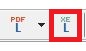
\includegraphics[width=1.2cm]{button-compiler-winedt.JPG}}图中红框内的按钮)完成第一遍\LaTeX 编译;
第二步,打开命令行(可以用winedt菜单accessories下command prompt项)输入命令biber filename完成参考文献数据准备;
第三步,再次点击xelatex编译按钮,完成编译,如果存在反向超链接,那么再次用xelatex编译一遍可以得到正确结果。

\subsubsection{利用texstudio}
texstudio可以多平台使用,在windows和linux下均可。texstudio可以通过利用元命令构建编译命令实现一键编译,进入选项菜单的设置texstudio项,首先在常规选项卡下设置语言为zh\_cn将texstudio界面语言转变为中文,然后在构建选项卡设置默认的编译器为xelatex,设置默认文献工具为biber(图\ref{texstudio:defaulttool}),然后点击构建并查看的配置按钮(\parbox{0.5cm}{\includegraphics[width=0.5cm]{texstudio-cmd-set.JPG}}),设置工具栏构建并查看按钮(\parbox{0.5cm}{
\includegraphics[width=0.5cm]{texstudio-cmd-build.JPG}})对应的命令由5个元命令构成(图\ref{texstudio:compilerchain})。这样点击构建并查看按钮即可完成一键编译功能。其编译的过程提示信息如例\ref{texstudio:onekeycompile}所示(环境为windows 7 x64+texlive 2016+tex studio 2.10.8)。

\begin{codetex}{texstudio一键编译过程提示}{texstudio:onekeycompile}
开始 : xelatex.exe -synctex=1 -interaction=nonstopmode "test".tex
完成

开始 : biber.exe "test"
INFO - This is Biber 2.5
INFO - Logfile is 'test.blg'
INFO - Reading 'test.bcf'
INFO - Found 0 citekeys in bib section 0
INFO - Found 4 citekeys in bib section 1
INFO - Found 0 citekeys in bib section 0
INFO - Processing section 1
INFO - Looking for bibtex format file 'example.bib' for section 1
INFO - Decoding LaTeX character macros into UTF-8
INFO - Found BibTeX data source 'example.bib'
WARN - Overwriting field 'year' with year value from field 'date' for entry '鍒樻捣娲013--'
WARN - Overwriting field 'year' with year value from field 'date' for entry '鑳′紵2011--'
WARN - BibTeX subsystem: C:\Users\ADMINI~1\AppData\Local\Temp\pru9Tr4B7_\example.bib_6592.utf8, line 1198, warning: possible runaway string started at line 1197
INFO - Overriding locale 'en-US' defaults 'normalization = NFD' with 'normalization = prenormalized'
INFO - Overriding locale 'en-US' defaults 'variable = shifted' with 'variable = non-ignorable'
INFO - Sorting list 'none/global/' of type 'entry' with scheme 'none' and locale 'en-US'
INFO - No sort tailoring available for locale 'en-US'
INFO - Writing 'test.bbl' with encoding 'UTF-8'
INFO - Output to test.bbl
INFO - WARNINGS: 3
完成

开始 : xelatex.exe -synctex=1 -interaction=nonstopmode "test".tex
完成

开始 : xelatex.exe -synctex=1 -interaction=nonstopmode "test".tex
完成
\end{codetex}


\begin{figure}[!htb]
  \centering
  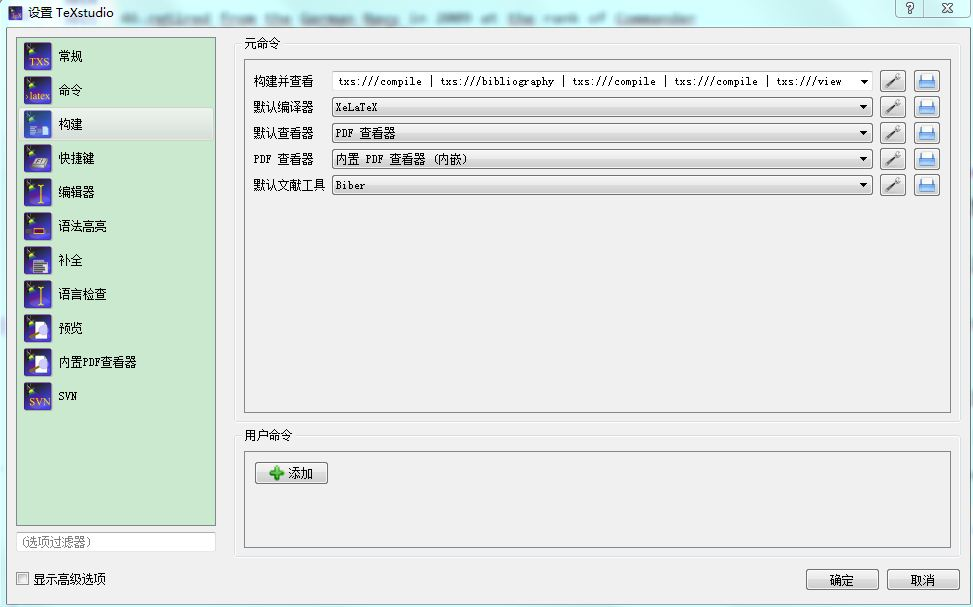
\includegraphics[width=\figwd\textwidth]{texstudio-defaulttool.JPG}
  \caption{texstudio设置默认的编译工具}\label{texstudio:defaulttool}
\end{figure}

\begin{figure}[!htb]
  \centering
  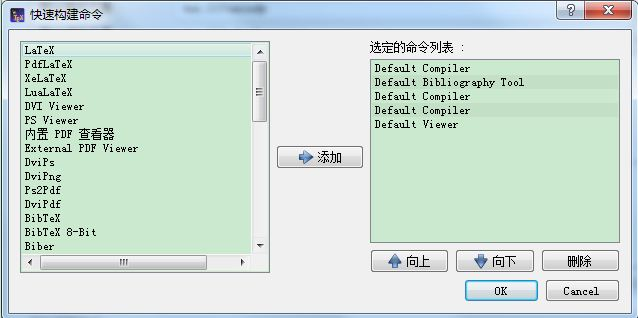
\includegraphics[width=\figwd\textwidth]{texstudio-compilerchain.JPG}
  \caption{texstudio配置构建并查看命令}\label{texstudio:compilerchain}
\end{figure}

linux(以deepin linux x64 v15+texlive 2016+texsudio为例)下texstudio的设置是类似的,但要正常编译还有一个关键问题需要设置即路径,这不是系统环境的路径设置,而是要告诉texstudio编译工具所在的路径,这同样在菜单选项下的设置texstudio项中设置,仍然进入构建选项卡,左下角点选显示高级选项,然后设置命令(\$PATH)为/usr/local/texlive/2016/bin/x86\_64-linux,如图\ref{texstudio:path:linux}所示。

\begin{figure}[!htb]
  \centering
  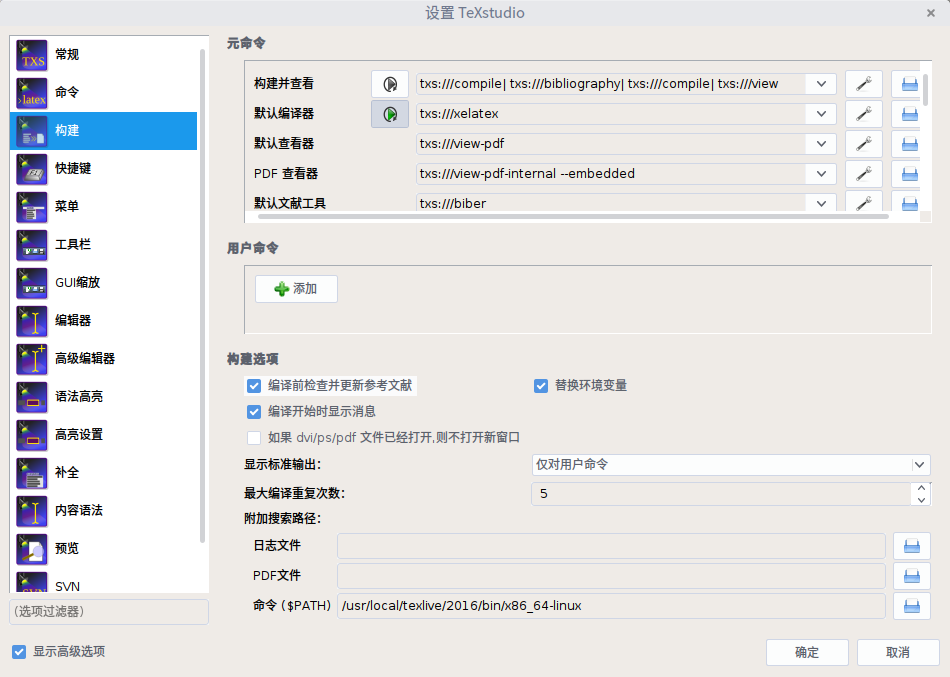
\includegraphics[width=\figwd\textwidth]{texstudio-path-linux.png}
  \caption{linux下texstudio设置命令路径}\label{texstudio:path:linux}
\end{figure}

\subsubsection{命令行或脚本}

命令行编译本质上是在命令行手动输入命令,命令过程仍然是一遍xelatex编译,biber编译,两边xelatex编译,命令如下:

\begin{codetex}{命令行手动输入的命令}{cmd:prompt}
xelatex.exe -synctex=1 -interaction=nonstopmode "test".tex
biber.exe "test"
xelatex.exe -synctex=1 -interaction=nonstopmode "test".tex
xelatex.exe -synctex=1 -interaction=nonstopmode "test".tex
\end{codetex}

利用脚本编译原理是一样的,只是利用编译脚本文件进行自动编译,注意:linux下的脚本文件需要添加一下路径。比如:
\begin{codetex}{window下的bat脚本文件}{bat:file:cmd}
@echo off
:: compile the tex file
xelatex.exe --synctex=-1 "test".tex
:: compile bibliography
biber "test"
:: compile again
xelatex.exe --synctex=-1 "test".tex
::to do it again for backref
xelatex.exe --synctex=-1 "test".tex
:: clear aux files
del /q *.aux *.bbl *.blg *.log *.out *.toc *.bcf *.xml *.synctex *.nlo *.nls *.bak *.ind *.idx *.ilg *.lof *.lot *.ent-x *.tmp *.ltx *.los *.lol *.loc *.listing *.gz
\end{codetex}

\begin{codetex}{linux下的sh脚本文件}{sh:file:cmd}
#!/bin/bash
# exec path for tex live 2016
export PATH=${PATH}:/usr/local/texlive/2016/bin/x86_64-linux

#compile the tex file
xelatex --synctex=-1 "test".tex
#compile bibliography
biber "test"
#compile again
xelatex --synctex=-1 "test".tex
#to do it again for backref
xelatex --synctex=-1 "test".tex
#clear aux files
rm -r *.aux *.bbl *.blg *.log *.out *.toc *.bcf *.xml *.synctex *.nlo *.nls *.bak *.ind *.idx *.ilg *.lof *.lot *.ent-x *.tmp *.ltx *.los *.lol *.loc *.listing *.gz
\end{codetex}

\subsection{分章参考文献和书后参考文献}
分章参考文献在书籍写作中是一种比较常见的需求。在latex传统方法中,利用thebibliography 环境可是实现,但其格式只能在bibitem内输入,对于文献量较大时是不适合的。而利用bibliographystyle 和 bibliography 命令生成的参考文献可以与thebibliography 环境同时存在,生成多个不同的文献表,可以插入多个文献表但却是相同的,这是因为编译文档时,所有的信息都是写入一个 aux 文件中的。所以要实现分章参考文献表,需要使用 chapterbib宏包,并且要把需要生成文献表的章放到单独的tex文件中,然后用include命令包含进主文件,这样可以生成多个aux文件以便生成分章参考文献表。而使用biblatex宏包可以很方便的在一个\LaTeX 文档中实现多种形式的参考文献划分,其中分章参考文献可以利用refsection环境或者宏包选项来实现。
\subsubsection{利用refsection环境分章}

利用refsection环境可以显式的设置需要打印参考文献的文档结构部分,比如把chapter的所有内容放在refsection环境内,那么在该refsection中使用参考文献打印命令printbibliography就会得到该环境内的参考文献信息,例\ref{bib:refsection}给出的代码,其结果如图\ref{bib:refsection:resa},\ref{bib:refsection:resb}所示。

\begin{codetex}{分章参考文献}{bib:refsection}
\documentclass{report}%%file:egrefsection.tex
\usepackage{ctex}
\usepackage[paperwidth=12cm,paperheight=6cm,top=0cm, bottom=1.5cm, left=1cm,right=1cm]{geometry}
\usepackage{titlesec}
\titleformat{\chapter}{\zihao{4}\heiti}{\thechapter}{1em}{}
\titlespacing*{\chapter}{0pt}{0.0\baselineskip}{0.5\baselineskip}[0pt]
\titleformat{\section}{\zihao{5}\heiti}{\thesection}{1em}{}
\titlespacing*{\section}{0pt}{0.5\baselineskip}{0.5\baselineskip}[0pt]
\usepackage[backend=biber,style=gb7714-2015]{biblatex}
\addbibresource[location=local]{example.bib}

\begin{document}
\chapter{序章}
\begin{refsection}
序章内容\cite{GPS1988--}
\printbibliography[heading=subbibliography,title=本章参考文献]
\end{refsection}

\chapter{正文章一}
\begin{refsection}
正文内容一\cite{杨洪升2013-56-75}
\printbibliography[heading=subbibliography,title=本章参考文献]
\end{refsection}

\chapter{正文章二}
\begin{refsection}
正文内容二\cite{马克思2013-302-302}
\printbibliography[heading=subbibliography,title=本章参考文献]
\end{refsection}
\end{document}
\end{codetex}

\begin{figure}[!htb]
  \centering
  \fbox{
\includegraphics[width=\figwd\textwidth,page=1]{egrefsection.pdf}}
  \caption{分章参考文献举例-序章}\label{bib:refsection:resa}
\end{figure}

\begin{figure}[!htb]
  \centering
  \fbox{
\includegraphics[width=\figwd\textwidth,page=2]{egrefsection.pdf}}
  \caption{分章参考文献举例-章一}\label{bib:refsection:resb}
\end{figure}

\subsubsection{利用宏包refsection选项分章}
除了利用refsection环境显式方法外,还可以利用宏包选项refsection=chapter等来设置需要区分打印参考文献的文档结构,这里设置refsection=chapter表示以章为单位区分打印参考文献,也可以设置成section,那么就是以节为单位进行区分打印。例\ref{bib:opt:refsection}给出的代码,其结果如图\ref{bib:refsection:resc}所示,可以看到与图\ref{bib:refsection:resa}完全一致。
\begin{codetex}{利用宏包选项实现分章参考文献}{bib:opt:refsection}
\documentclass{report}%%file:egrefsectionb.tex
\usepackage{ctex}
\usepackage[paperwidth=12cm,paperheight=6cm,top=0cm, bottom=1.5cm, left=1cm,right=1cm]{geometry}
\usepackage{titlesec}
\titleformat{\chapter}{\zihao{4}\heiti}{\thechapter}{1em}{}
\titlespacing*{\chapter}{0pt}{0.0\baselineskip}{0.5\baselineskip}[0pt]
\titleformat{\section}{\zihao{5}\heiti}{\thesection}{1em}{}
\titlespacing*{\section}{0pt}{0.5\baselineskip}{0.5\baselineskip}[0pt]
\usepackage[backend=biber,refsection=chapter,style=gb7714-2015]{biblatex}
\addbibresource[location=local]{example.bib}

\begin{document}
\chapter{序章}
序章内容\cite{GPS1988--}
\printbibliography[heading=subbibliography,title=本章参考文献]

\chapter{正文章一}
正文内容一\cite{杨洪升2013-56-75}
\printbibliography[heading=subbibliography,title=本章参考文献]

\chapter{正文章二}
正文内容二\cite{马克思2013-302-302}
\printbibliography[heading=subbibliography,title=本章参考文献]
\end{document}
\end{codetex}

\begin{figure}[!htb]
  \centering
  \fbox{
\includegraphics[width=\figwd\textwidth,page=1]{egrefsectionb.pdf}}
  \caption{设置宏包选项实现分章参考文献}\label{bib:refsection:resc}
\end{figure}

\subsubsection{统一的全局参考文献}

biblatex参考文献利用refsection很容易生成分章节的参考文献,但如果要生成一个全局的参考文献,那么可以不使用任何的refsection或者使用一个refsection包含全部的文档(注意:两种方法对于一般情况下都是可以的,但第二种方法对于beamer类则不能使用,这在第\ref{sec:bib:inbeamer}节还要详说)。

但还有一种情况是既要生成分章参考文献又要有一个全局的参考文献。那么最简单的方式在文末利用printbibliography的section选项对所有的refsection同时打印一遍,代码如例\ref{bib:global:refsection}所示,但这样的方式更像是文献表堆积,不像一个统一的文献表,且其中的各章的文献引用标注序号不是全局的,只是各refsection内部的序号。

\begin{codetex}{利用refsection的全局参考文献}{bib:global:refsection}
\printbibliography[section=1,heading=subbibliography,title=第一章参考文献]
\printbibliography[section=2,heading=subbibliography,title=第二章参考文献]
\printbibliography[section=3,heading=subbibliography,title=第三章参考文献]
\end{document}
\end{codetex}

这个问题可以用refsegment代替refsection来解决。refsegment与refsection作用很像也用于划分,但其内部的文献序号是全文统一的。每一个segment都有一个编号从1开始,用printbibliography命令打印在某个refsegment环境内的使用参考文献,只需要给出segment=整数的一个值,该值表示第几个refsegment环境。而在refsegment环境外的参考文献默认在segment=0的segment内,若printbibliography命令中给出segment=0则打印不在任一refsegment环境内的文献,若不给出segment参数则遍历所有可以打印的参考文献,包括各个refsegment内的文献。

(注意:refsection内部可以有refsection,即refsection不可嵌套,但其内部可以使用refsegment。printbibliography命令也可以对refsection内的所有refsegment遍历打印,也可以指定refsection内的某一个refsegment中的文献,只要各处segment参数,当printbibliography在refsection外打印其内refsegment中的文献,则还需要指定section参数。

例\ref{eg:global:complex}给出一个测试代码,其结果如图\ref{fig:eg:global:complex}所示。其中“文献全局”命令遍历打印了所有不在refsection内的文献,包括refSegment A,refSegment B,以及不在其内的Gradshteyn和附录的Section E中的Parsons文献。
\begin{codetex}{全局参考文献综合示例}{eg:global:complex}
%file:egbibdiv.tex
\documentclass{article}
\usepackage{ctex,hyperref}
\usepackage{geometry}
\geometry{paperwidth=21cm,paperheight=26cm,%
left=1cm,right=1cm,top=1cm,bottom=1.5cm}
\usepackage[backend=biber,style=gb7714-2015]{biblatex}
\addbibresource{example.bib}
\renewcommand{\bibfont}{\zihao{6}}
\usepackage{titlesec}
%\titleformat{command}[shape]{format}{label}{sep}{before}[after]
\titleformat{\section}{\centering\bfseries}{第\thesection 节}{1em}{}[]
\titlespacing*{\section}{0pt}{0.0\baselineskip}{0.0\baselineskip}[0pt]
\titleformat{\subsection}{\flushleft\bfseries}{\S\,\thesubsection}{1em}{}[]
\titlespacing*{\subsection}{0pt}{0.0\baselineskip}{0.0\baselineskip}[0pt]
\begin{document}
\small 	参考文献测试\cite{Gradshteyn2000--}。
	\begin{refsegment}
		\section{refSegment A}
		分章节参考文献测试\cite{Chiani2003-840-845}
		\printbibliography[segment=1,heading=subbibliography,title=文献A]
	\end{refsegment}
	
	\begin{refsegment}
		\section{refSegment B}
		参考文献测试\cite{张敏莉2007-500-503}
	\end{refsegment}
	%\printbibliography放在refsegment环境外也是可以的
	\printbibliography[segment=2,heading=subbibliography,title=文献B]
	
	\begin{refsection}
		\section{refsection C}
		参考文献测试\cite{Zhang2007-500-503}
	\end{refsection}

	\begin{refsection}
		\section{refsection D}
		分章节参考文献测试\cite{Andersen1995-42-49}
    	\begin{refsegment}
			\subsection{refsegment D-1}
			分章节参考文献测试\cite{Simon2004--}。
		\end{refsegment}
		\begin{refsegment}
			\subsection{refsegment D-2}
			分章节参考文献测试\cite{Lin2004--}。
		\end{refsegment}
	\end{refsection}
    \printbibliography[section=2,segment=0,heading=subbibliography,title=文献D0]
    \printbibliography[section=2,segment=1,heading=subbibliography,title=文献D1]
    \printbibliography[section=2,segment=2,heading=subbibliography,title=文献D2]
	\printbibliography[section=1,heading=subbibliography,title=文献C]
    \printbibliography[section=2,heading=subbibliography,title=文献D]
	%遍历非refsection内的参考文献
	\printbibliography[heading=bibliography,title=文献全局]
	\appendix
	\section{Section E}
	参考文献测试\cite{Parsons2000--}。
\end{document}
\end{codetex}

\begin{figure}[!htb]
	\centering
	% Requires \usepackage{graphicx}
	
\includegraphics[width=0.9\linewidth]{egbibdiv.pdf}\\
	\caption{全局参考文献综合示例}\label{fig:eg:global:complex}
\end{figure}


\subsection{参考文献标题格式}
要投稿的文章经常需要设置某种格式的参考文献标题,包括字号,大小,段落格式等。在书籍等写作中有时还需要将参考文献加入目录中,以便实现超链接。
\subsubsection{加入目录链接}

加入目录的命令是addcontentsline,在printbibliography命令前使用该命令即可将参考文献加入目录中,同时为了能够超链接正确可以加入hyperref宏包提供的phantomsection命令。例\ref{bib:inserttoc}给出了代码。
\begin{codetex}{手动加入目录链接}{bib:inserttoc}
\addcontentsline{toc}{chapter}{参考文献}
\phantomsection
\printbibliography[heading=bibliography,title=本章参考文献]
\end{codetex}

除了上述手动添加的方式外,还可以在printbibliography命令使用biblatex提供的选项来实现,比如heading=bibintoc,该选项与heading=bibliography是类似的,只是增加了在目录中加入链接的功能,例\ref{bib:inserttoc:bibintoc}给出了代码。
\begin{codetex}{使用bibintoc加入目录链接}{bib:inserttoc:bibintoc}
\printbibliography[heading=bibintoc,title=本章参考文献]
\end{codetex}

\subsubsection{重定义heading}

默认情况下,biblatex参考文献标题的格式主要依赖于\LaTeX 文档的章节的标题格式。当printbibliography中使用heading选项的参数是bibliography和bibintoc时,参考文献标题的格式与当前文档类的主划分单元的标题格式一致,比如book和report类中与chapter一致,而在article类中与section一致。heading选项的参数是subbibliography和subbibintoc时,则是主单元的下一层级的标题格式一致,即book和report类中与section一致,而在article类中与subsection一致。因此设置参考文献标题的格式最简单方式是设置文档的各级标题格式然后选择heading选项的参数(注意当heading选项不给出时,其默认参数为bibliography)。

事实上利用defbibheading命令重定义bibliography等选项的信息,改变默认的标题对应方式,比如可以将bibliography与subsubsection层级标题格式对应起来,例\ref{bib:def:headsec}给出了代码。其中还使用了phantomsection和addcontentsline命令可以完成上一小节需要的加入目录链接功能。其中还使用了centering使标题居中,这预示了一种标题格式修改方式,甚至可以不使用文档类的标题格式而直接自定义标题。

\begin{codetex}{biblatex对于目录的影响}{bib:def:headsec}
\usepackage[backend=biber,style=gb7714-2015ay]{biblatex}
\defbibheading{bibliography}[\bibname]{%
\phantomsection%解决链接指引出错的问题,相当于加入了一个引导点
\addcontentsline{toc}{subsubsection}{#1}
	\centering\subsubsection*{#1}}%
\end{codetex}

需要注意,如果要使用titleps作为页眉页脚的设置宏包,那么需要利用defbibheading重设一下heading选项参数,因为默认情况下heading的参数比如bibliography中带有markboth命令,该命令与titleps共用时会导致页眉页脚一些出现问题。例\ref{bib:def:heading}给出了代码。而使用文档类默认的页眉页脚或者利用fancyhdr设置页眉页脚,则不需要修改。为了方便移植应用,这里给出三种设置页眉页脚的代码,例\ref{head:class:ctex}是使用文档类提供和ctex修改的页眉页脚;例\ref{head:fancyhdr}是使用fancyhdr设置的页眉页脚;例\ref{head:titleps}是使用titleps设置的页眉页脚。

\begin{codetex}{重设heading选项参数}{bib:def:heading}
\defbibheading{bibliography}[\bibname]{%
	\chapter*{#1}}%
%	\markboth{#1}{#1}}
%重定义命令中去掉了markboth那一句命令。
\end{codetex}

\begin{codetex}{文档类提供ctex修改的页眉页脚举例}{head:class:ctex}
%file:egheadclass.tex
\documentclass{book}
\usepackage{ctex}
\usepackage[paperwidth=12cm,paperheight=6cm,top=1.5cm, bottom=1.5cm, left=1cm,right=1cm]{geometry}
\usepackage{titlesec}
\titleformat{\chapter}{\zihao{4}\heiti}{\thechapter}{1em}{}
\titlespacing*{\chapter}{0pt}{0.0\baselineskip}{0.5\baselineskip}[0pt]
\titleformat{\section}{\zihao{5}\heiti}{\thesection}{1em}{}
\titlespacing*{\section}{0pt}{0.5\baselineskip}{0.5\baselineskip}[0pt]
\usepackage[backend=biber,style=nature]{biblatex}
\addbibresource[location=local]{example.bib}

\renewcommand{\bibfont}{\zihao{-6}\songti}
\setlength{\bibitemsep}{2pt}
\usepackage{hyperref}
\begin{document}
\tableofcontents
\begin{refsection}
\chapter{序章}
\section{序节}
序章内容\cite{GPS1988--}
\defbibentryset{bilangyi2013}{易仕和2013--,Yi2013--}
专著,双语文献引用\cite{bilangyi2013}

\phantomsection
\addcontentsline{toc}{chapter}{参考文献}
\printbibliography[heading=bibliography,title=本章参考文献]
\end{refsection}

\begin{refsection}
\chapter{正文章一}
\section{正文节一}
正文内容一\cite{杨洪升2013-56-75}

\phantomsection
\addcontentsline{toc}{section}{参考文献}
\printbibliography[heading=subbibliography,title=本章参考文献]
\end{refsection}

\begin{refsection}
\chapter{正文章二}
\section{正文节二}

正文内容二\cite{马克思2013-302-302}
\printbibliography[heading=subbibliography,title=本章参考文献]
\end{refsection}
\end{document}
\end{codetex}

\begin{codetex}{利用fancyhdr生成页眉页脚举例}{head:fancyhdr}
%file:egheadfancy.tex
\documentclass{book}
\usepackage{ctex}
\usepackage[paperwidth=12cm,paperheight=6cm,top=1.5cm, bottom=1.5cm, left=1cm,right=1cm]{geometry}
\usepackage{titlesec}
\titleformat{\chapter}{\zihao{4}\heiti}{\thechapter}{1em}{}
\titlespacing*{\chapter}{0pt}{0.0\baselineskip}{0.5\baselineskip}[0pt]
\titleformat{\section}{\zihao{5}\heiti}{\thesection}{1em}{}
\titlespacing*{\section}{0pt}{0.5\baselineskip}{0.5\baselineskip}[0pt]
\usepackage[backend=biber,style=nature]{biblatex}
\addbibresource[location=local]{example.bib}

\renewcommand{\bibfont}{\zihao{-6}\songti}
\setlength{\bibitemsep}{2pt}
\usepackage{hyperref}
\usepackage{fancyhdr}
\pagestyle{fancy}
\renewcommand{\chaptermark}[1]{%
\markboth{#1}{}}
\renewcommand{\sectionmark}[1]{%
\markright{\thesection\ #1}}
\fancyhf{} % delete current header and footer
\fancyhead[LE,RO]{\bfseries\thepage}
\fancyhead[LO]{\bfseries\rightmark}
\fancyhead[RE]{\bfseries\leftmark}
\renewcommand{\headrulewidth}{0.5pt}
\renewcommand{\footrulewidth}{0pt}
\addtolength{\headheight}{0.5pt} % space for the rule
\fancypagestyle{plain}{%
\fancyhead{} % get rid of headers on plain pages
\renewcommand{\headrulewidth}{0pt} % and the line
}

\begin{document}
\tableofcontents
\begin{refsection}
\chapter{序章}
\section{序节}
序章内容\cite{GPS1988--}
\defbibentryset{bilangyi2013}{易仕和2013--,Yi2013--}
专著,双语文献引用\cite{bilangyi2013}

\phantomsection
\addcontentsline{toc}{chapter}{参考文献}
\printbibliography[heading=bibliography,title=本章参考文献]
\end{refsection}

\begin{refsection}
\chapter{正文章一}
\section{正文节一}
正文内容一\cite{杨洪升2013-56-75}

\phantomsection
\addcontentsline{toc}{section}{参考文献}
\printbibliography[heading=subbibliography,title=本章参考文献]
\end{refsection}

\begin{refsection}
\chapter{正文章二}
\section{正文节二}
正文内容二\cite{马克思2013-302-302}
\printbibliography[heading=subbibliography,title=本章参考文献]
\end{refsection}
\end{document}
\end{codetex}

\begin{codetex}{利用titleps生成页眉页脚举例}{head:titleps}
%file:egheadtitleps.tex
\documentclass{book}
\usepackage{ctex}
\usepackage[paperwidth=12cm,paperheight=6cm,top=1.5cm, bottom=1.5cm, left=1cm,right=1cm]{geometry}
\usepackage[pagestyles]{titlesec}
\titleformat{\chapter}{\zihao{4}\heiti}{\thechapter}{1em}{}
\titlespacing*{\chapter}{0pt}{-1.0\baselineskip}{0.5\baselineskip}[0pt]
\titleformat{\section}{\zihao{5}\heiti}{\thesection}{1em}{}
\titlespacing*{\section}{0pt}{0.5\baselineskip}{0.5\baselineskip}[0pt]
\usepackage[backend=biber,style=nature]{biblatex}
\addbibresource[location=local]{example.bib}

\renewcommand{\bibfont}{\zihao{-6}\songti}
\setlength{\bibitemsep}{2pt}
\defbibheading{bibliography}[\bibname]{%
\phantomsection%
\addcontentsline{toc}{chapter}{#1}%
\chapter*{#1}}%
\defbibheading{subbibliography}[\bibname]{%
\phantomsection%
\addcontentsline{toc}{section}{#1}%
\section*{#1}}%
\usepackage{hyperref}

\newpagestyle{main}{%偶数页
\sethead[\small$\cdot$~\thepage~$\cdot$][]
[\small\,\thesection\quad\sectiontitle]%奇数页
{\small\,\thechapter\quad\chaptertitle}{}{\small$\cdot$~\thepage~$\cdot$}
\setfoot{}{}{}\headrule\footrule}
%注意\sectiontitle应该是titlesec宏包定义的命令
\renewcommand\headrule{\setheadrule{1pt}}
\renewcommand\footrule{\setfootrule{0pt}}

\newpagestyle{premain}{
\sethead[\small$\cdot$~\thepage~$\cdot$][][\small\,目录]
{\small\,\leftmark}{}{$\cdot$~\thepage~$\cdot$}
\setfoot{}{}{}\headrule\footrule}

\newpagestyle{pgref}{%
	\sethead[\small\,~\thepage~]% 偶数页左
	[]% 偶数页中
	[\small\,参考文献]% 偶数页右
	{\small\,\thechapter\quad\chaptertitle\hfil}% 奇数页左
	{}% 奇数页中
	{\small\,~\thepage~}% 奇数页右
	\setfoot{}{}{}%
	\headrule%
}%

\begin{document}
\pagestyle{premain}
\tableofcontents
\cleardoublepage

\begin{refsection}
\pagestyle{main}
\chapter{序章}
\section{序节}
序章内容\cite{GPS1988--}
\defbibentryset{bilangyi2013}{易仕和2013--,Yi2013--}
专著,双语文献引用\cite{bilangyi2013}
%\newpage
%\vfil\hspace{1pt}
%\newpage
\pagestyle{pgref}
\printbibliography[heading=bibliography,title=本章参考文献]
\cleardoublepage%页眉页脚分割正确需要该命令
\end{refsection}

\begin{refsection}
\pagestyle{main}
\chapter{正文章一}
\section{正文节一}
正文内容一\cite{杨洪升2013-56-75}
%\newpage
%\vfil\hspace{1pt}
%\newpage
\pagestyle{pgref}
\printbibliography[heading=subbibliography,title=本章参考文献]
\cleardoublepage
\end{refsection}

\begin{refsection}
\pagestyle{main}
\chapter{正文章二}
\section{正文节二}
正文内容二\cite{马克思2013-302-302}
%\newpage
%\vfil\hspace{1pt}
%\newpage
\pagestyle{pgref}
\printbibliography[heading=subbibliography,title=本章参考文献]
\cleardoublepage
\end{refsection}
\end{document}
\end{codetex}

\subsubsection{利用titlesec}

既然参考文献的标题可以使用文档类的标题格式,且titlesec的标题样式命令具有局部性命令具有局部性,那么完全可以利用titlesec宏包定义一个需要的标题格式,在参考文献使用完以后然后恢复原来的设置。(注意: 当使用titlesec宏包重定义section等标题样式后,在defbibheading命令中使用centering可能无效)。例\ref{sec:md:titlesec}给出了测试代码,其结果如图\ref{bib:sec:md}所示。

\begin{codetex}{利用titlesec局部修改参考文献标题格式}{sec:md:titlesec}
%file:egsectitle.tex
\documentclass{book}
\usepackage{ctex}
\usepackage[paperwidth=12cm,paperheight=7cm,top=1.5cm, bottom=1.5cm, left=1cm,right=1cm]{geometry}
%注意页面高度太小的话,可能会使[openright]失效,原因待研
%这里设置paperheight=6或者5都会使第一章开启页不在奇数页
\usepackage{xcolor}
\usepackage[pagestyles]{titlesec}
\usepackage{titletoc}
\titleformat{\chapter}{\zihao{4}\heiti}{\thechapter}{1em}{}
\titlespacing*{\chapter}{0pt}{0.0\baselineskip}{0.5\baselineskip}[0pt]
\titleformat{\section}{\zihao{5}\heiti}{\thesection}{1em}{}
\titlespacing*{\section}{0pt}{0.5\baselineskip}{0.5\baselineskip}[0pt]
\usepackage[backend=biber,style=gb7714-2015]{biblatex}
\addbibresource[location=local]{example.bib}
\defbibheading{subbibliography}[\bibname]{%
\section{#1}}%
\renewcommand{\bibfont}{\zihao{-6}\songti}
\setlength{\bibitemsep}{2pt}
\usepackage{hyperref}

\begin{document}
\tableofcontents

\begin{refsection}
\chapter{序章}
\titleformat{\section}[frame]{\normalfont}{\filright\footnotesize\enspace SECTION \thesection\enspace}
{8pt}{\bfseries\filcenter}
\section{序节}
序章内容\cite{GPS1988--}
\printbibliography[heading=subbibliography,title=本章参考文献]
\end{refsection}

\begin{refsection}
\chapter{正文章一}
\section{正文节一}
正文内容一\cite{杨洪升2013-56-75}
\printbibliography[heading=subbibliography,title=本章参考文献]
\end{refsection}
\end{document}
\end{codetex}

\begin{figure}[!htb]
  \centering
  \fbox{\includegraphics[width=\figwd\textwidth,page=4]{egsectitle.pdf}}
  \caption{利用titlesec局部修改参考文献标题格式}\label{bib:sec:md}
\end{figure}


\subsection{参考文献内容格式}

参考文献内容格式的格式可以重定义biblatex宏包提供的命令来实现。

\subsubsection{一般设置方法}

字体字号由钩子命令bibfont设置,垂直间距由bibitemsep、bibnamesep、bibinitsep三个尺寸进行设置,bibitemsep表示每一条参考文献之间的间隔,bibnamesep表示当本条文献与前一条文献的责任者不同时设置的间隔,bibinitsep表示本条文献与前一条文献的首字母不同时设置的间隔(注意:当设置排序sorting=none的时候,bibinitsep的作用有所变化),一般情况下使用bibitemsep,bibnamesep已然足够,需要注意这三个尺寸遵守addvspace的规则,同时存在时取最大的那个尺寸作为间隔。设置的方式如例\ref{bib:font:set}所示:

\begin{codetex}{参考文献表内容的格式}{bib:font:set}
%参考文献文本字体为默认字体,字号为小五,利用ctex设置
%如果不是利用ctex宏包,可以利用其它字号设置命令
\renewcommand{\bibfont}{\zihao{6}}
%设置各条参考文献之间的间距为0pt
\setlength{\bibitemsep}{0pt}
%\setlength{\bibnamesep}{1ex}
%\setlength{\bibinitsep}{2ex}
\end{codetex}

\subsubsection{自定义环境和局部修改}
参考文献表是有biblatex或者样式包提供的参考文献表环境打印和控制的,通常是由list环境自定义而来,所以要设置参考文献表的内容的段落格式,需要从修改参考文献表环境defbibenvironment\{bibliography\}入手,通常情况这是不需要去做的,由所选的样式包设置即可。如果有特殊的需求可以自定义一个参考文献表环境来控制其格式。如果使用list通用环境作为基础环境来定义的话,其段落格式的参数设置可以参考文献\pagescite[][74-80]{Kopka2004--}\pagescite[][265-268]{Braams2015--}。注意到其实latex中的很多环境比如center,quote等都是由通用list环境所定义的。

同时,因为bibfont等命令的使用具有局部性,所以可以在文档中多次定义,用于打印不同效果的文献表。例\ref{bib:fontset:eg}给出一个完成的测试代码,其中打印了4个参考文献表,分别用了不同的字体。同时设置了bibitemsep、bibnamesep、bibinitsep三个尺寸控制各条文献的间距。并且自定义了一个参考文献表环境marginref,并没有使用list环境,而是简单的编组后打印环境,可以看到其中各条文献的缩进效果。

\begin{codetex}{参考文献表内容格式修改举例}{bib:fontset:eg}
%file:egbibfont.tex
\documentclass{report}
\usepackage{ctex}
\usepackage{geometry}
\geometry{paperwidth=15cm,paperheight=12cm,top=0cm, bottom=1.5cm, left=1cm,right=1cm}
\usepackage{titlesec}
\titleformat{\chapter}{\zihao{5}\heiti}{\thechapter}{1em}{}
\titlespacing*{\chapter}{0pt}{0.0\baselineskip}{0.0\baselineskip}[0pt]
\titleformat{\section}{\zihao{-5}\heiti}{\thesection}{1em}{}
\titlespacing*{\section}{0pt}{0.0\baselineskip}{0.0\baselineskip}[0pt]
\usepackage[backend=biber,style=gb7714-2015]{biblatex}%sorting=none,
\addbibresource[location=local]{example.bib}

\usepackage{fontspec}
\newcommand{\ftArial}{\fontspec{Arial}\selectfont}
\newcommand{\ftcouriernew}{\fontspec{Courier New}\selectfont}
%参考文献文本字体设置为默认,字号为6,利用ctex设置
%如果不是利用ctex宏包,可以利用其它字号设置命令
\renewcommand{\bibfont}{\zihao{6}}
%设置各条参考文献之间的间距为0pt
\setlength{\bibitemsep}{0pt}
\setlength{\bibnamesep}{1ex}
\setlength{\bibinitsep}{2ex}

\newcommand{\itemcmd}[1]{#1\par}
\defbibenvironment{marginref}{\begingroup
\renewcommand{\baselinestretch}{0.8}
%\setlength{\parindent}{0pt}
\setlength{\parskip}{0pt}}
{\endgroup\clearpage}{\itemcmd}%\newline

\begin{document}
\chapter{序章}
\section{序节}
\tiny
序章内容\cite{GPS1988--,杨洪升2013-56-75,马克思2013-302-302}
正文内容一\cite{Andersen1995-42-49,BUSECK1980-117-211,Calkin2011-8-9}
正文内容二\cite{Parsons2000b--,Parsons2000--,Parsons2000noloc--,Parsons2000nodate--}
\printbibliography[heading=subbibliography,title=参考文献]
\newpage
\renewcommand{\bibfont}{\zihao{6}\ftArial\fangsong}
\printbibliography[heading=subbibliography,title=参考文献]
\newpage
\renewcommand{\bibfont}{\zihao{6}\ttfamily}
\printbibliography[heading=subbibliography,title=参考文献]
\newpage
\renewcommand{\bibfont}{\zihao{6}\ftcouriernew\kaishu}
\printbibliography[env=marginref,heading=subbibliography,title=参考文献]
\end{document}
\end{codetex}

第一个文献表如图\ref{bib:font:normal}所示,使用的是默认字体即宋体。第二个文献表如图\ref{bib:font:fs}所示,使用字体是Arial和仿宋。第三个文献表如图\ref{bib:font:tt}所示,使用的是默认字体的等宽字体。第四个文献表如图\ref{bib:font:kt}所示,使用的是Courier New和楷书字体,同时文献表环境是自定义的。(注意:因为linux下没有Arial和Courier New字体,所以用texlive自带的字体替换,linux下使用texlive自带的字体需要特殊设置,详见\pagescite[][15-16]{Berry2016--})。

\begin{figure}[!htb]
  \centering
  \fbox{
\includegraphics[width=0.85\textwidth,page=1]{egbibfont.pdf}}
  \caption{参考文献表格式默认字体字号六}\label{bib:font:normal}
\end{figure}

\begin{figure}[!htb]
  \centering
  \fbox{
\includegraphics[width=0.85\textwidth,page=2]{egbibfont.pdf}}
  \caption{参考文献表格式仿宋字体字号六}\label{bib:font:fs}
\end{figure}

\begin{figure}[!htb]
  \centering
  \fbox{
\includegraphics[width=0.85\textwidth,page=3]{egbibfont.pdf}}
  \caption{参考文献表格式等宽字体字号六}\label{bib:font:tt}
\end{figure}

\begin{figure}[!htb]
  \centering
  \fbox{
\includegraphics[width=0.85\textwidth,page=4]{egbibfont.pdf}}
  \caption{参考文献表格式楷书字体字号六}\label{bib:font:kt}
\end{figure}

\subsection{参考文献著录和标注样式}
参考文献著录和标注样式是排版的主要内容之一,但对于普通用户来说只要学会选择使用即可,因为其格式已经由样式作者所设定。当然如果用户需要在某种样式的基础上有进一步的修改,那么可以做这方面的工作。其中著录样式的在*.bbx文件中修改,而标注样式在*.cbx文件中修改。
\subsubsection{标准样式}
biblatex提供了一些标准的样式,比如numeric,authoryear,这两个样式是比较常用的,也是样式作者定制某种样式的重要基础。biblatex还提供了更多著录样式,比如alphabetic,authortitle,verbose等,详见biblatex手册Bibliography Styles一节。标注样式也还有numeric-comp,numeric-verb,alphabetic,authortitle等,详见biblatex手册Citation Styles一节。

\subsubsection{gb7714-2015}
本文的作者在学习GB/T 7714-2015标准的基础上,定制了符合该标准的gb7714-2015样式包,分顺序制和作者年制两类。其加载方式见例\ref{code:pkg:load}。

样式包的主要特点包括:
\begin{enumerate}
  \item 实现了GB/T 7714-2015标准的完整功能,不仅包括两种编制方式下的各类型参考文献著录格式和标注格式等基本功能,还包括:双语文献格式,带页码的标注格式,作者年制下文献的自动排序和仅有年的标注格式,两种编码制方式下责任者缺省不同处理,其他信息缺省时的自动处理,一些信息如页码卷期等自动解析等特殊功能。
  \item 实现了用户文献数据录入优化,用户在录入参考文献数据的时候,只需要录入文献的实际信息即可,不需要录入文献标识符和载体标识符,不需要录入language或者其它域信息用来区分中英文文献,完全实现自动中英文判断并处理。仅需要针对报纸文章和标准文章在note域输入news和standard 用以区分。
  \item 实现了对biblatex不同版本的兼容,能够应用于biblatex3.2以前的老版本,也能用于3.3以后姓名处理方式改变后的版本。即可以与texlive2014/2015/2016配合使用,无需升级biblatex情况下安装biblatex-gb7714-2015宏包即可使用。
  \item 使用文档详细介绍了各种条目类型的著录格式及其在biblatex中对应域的构成,说明了域信息的录入方法和一些注意点,说明了样式文件的使用方法和注意事项,并严格按照GB/T 7714-2015标准测试了各种类型的文献。
\end{enumerate}

关于参考文献数据录入准备、条目类型的域构成、样式包使用说明等更多的内容详见\cite{胡振震2016}。

biblatex-gb7714-2015样式宏包可以使用tlmgr或离线方式安装。
在texlive 2016下,使用tlmgr比较方便,步骤如下:

(a) 打开tlmgr-gui,在选项通用里面设置中国的ctan镜像源,比如\url{http://mirrors.ustc.edu.cn/CTAN/systems/texlive/tlnet}

(b) 点击,加载缺省软件包仓库。加载完成后可能要求升级tlmgr,那么先升级tlmgr。

(c) 在完成加载后,在匹配文本框填入biblatex-gb7714-2015,搜索安装即可。

这与安装其他宏包原理是一样的。

在texlive 2014 / texlive2015 下使用如下步骤:

(a) 在ctan上面下载biblatex-gb7714-2015宏包,下载地址:https://www.ctan.org/pkg/biblatex-gb7714-2015

(b) 解压压缩包,放到:texlive的texmf-dist/tex/latex或者texmf-local/tex/latex或者它们的子目录下面。(参考:texlive-zh-cn.pdf的3.4.6节)

(c) 运行texhash或者mktexlsr命令,刷新文件名数据库。

texlive 2016 当然也可以用这种方式离线安装。

\subsubsection{其他定制样式}
在texlive安装包或者ctan上面可以找到更多的定制样式,有针对某些期刊的文献样式比如nature,science,nejm等等,有些是作者自己兴趣所做比如:biblatex-caspervector样式包,该包作者本来是根据GB/T 7714-2005做的样式,后进一步形成了自己喜欢的风格。用户可以测试各样式包,并按需使用,进一步也可以参考其代码,修改自己需要的样式。

总的来说,因为biblatex提供了参考文献数据的完全访问能力,所以定义任何需要的样式都是可能的。因此用户可以根据需要对选择使用合适的样式或者定制需要的样式。

\subsubsection{快速定制/临时定制}
有的时候对于参考文献格式会有一些特殊的需求,而且往往这些格式并没有一个对应能够满足其要求的参考文献样式包,这种情况下就需要进行定制,比如\cite{olqa2016--}提出的问题。在latex传统方法中,当文献量较小时,这种临时定制采用thebibliography环境是比较方便的,因为thebibliography 环境显式的将其中的内容插入,因此需要什么样的格式,那么就在bibitem中输入指定格式的条目内容即可。但该环境存在一个问题即:无论引用与否环境中的参考文献都会全部打印。该环境也可以用来生成多个参考文献表,当然文献量较大时还采用这种手动输入方式毕竟是不方便的。

事实上利用biblatex可以实现快速的定制,biblatex宏包使用手册的Bibliography Style Files给出了样式文件定义的一般模式和方法。依据该模式是容易实现样式快速定制的,因为在一般情况下定制样式文件,其实并不需要处理太多的内容。总结起来,定制简单的参考文献格式需要处理的主要内容包括:
\begin{enumerate}
  \item 加载定制所需的基础样式比如标准样式或其它样式
  \item 设置宏包选项
  \item 设置单元或块的标点
  \item 设置域格式
  \item 设置驱动格式
\end{enumerate}
当然对于一些复杂的参考文献样式(比如gb7714-2015)还需要处理更多的内容,包括:
\begin{enumerate}
  \item 增加和应用需要的判断和函数
  \item 动态数据处理
  \item 增加一些域格式,增加修改应用本地化字符等
\end{enumerate}
在上述ctex论坛上的提问中,参考文献格式主要需要修改的内容是分块、分块的标点、分块内容的格式。其中: 作者是一个块作为一行,标题是一个块作为一行,其它是一个块作为一行,那么把块标点设置为换行,就可以实现多行。同时各块的内容的字体不同,作者是粗体,标题是等宽,其它是斜体,那么把对应的块所构成域的格式改成需要的格式即可。这里给出该问题的一个简单解答,如图\ref{bib:style}所示。采用的样式文件代码如例\ref{bib:style:customize}所示,其中为了简化修改,把一些条目设置成了相同的格式。

\begin{figure}[!htb]
  \centering
  \fbox{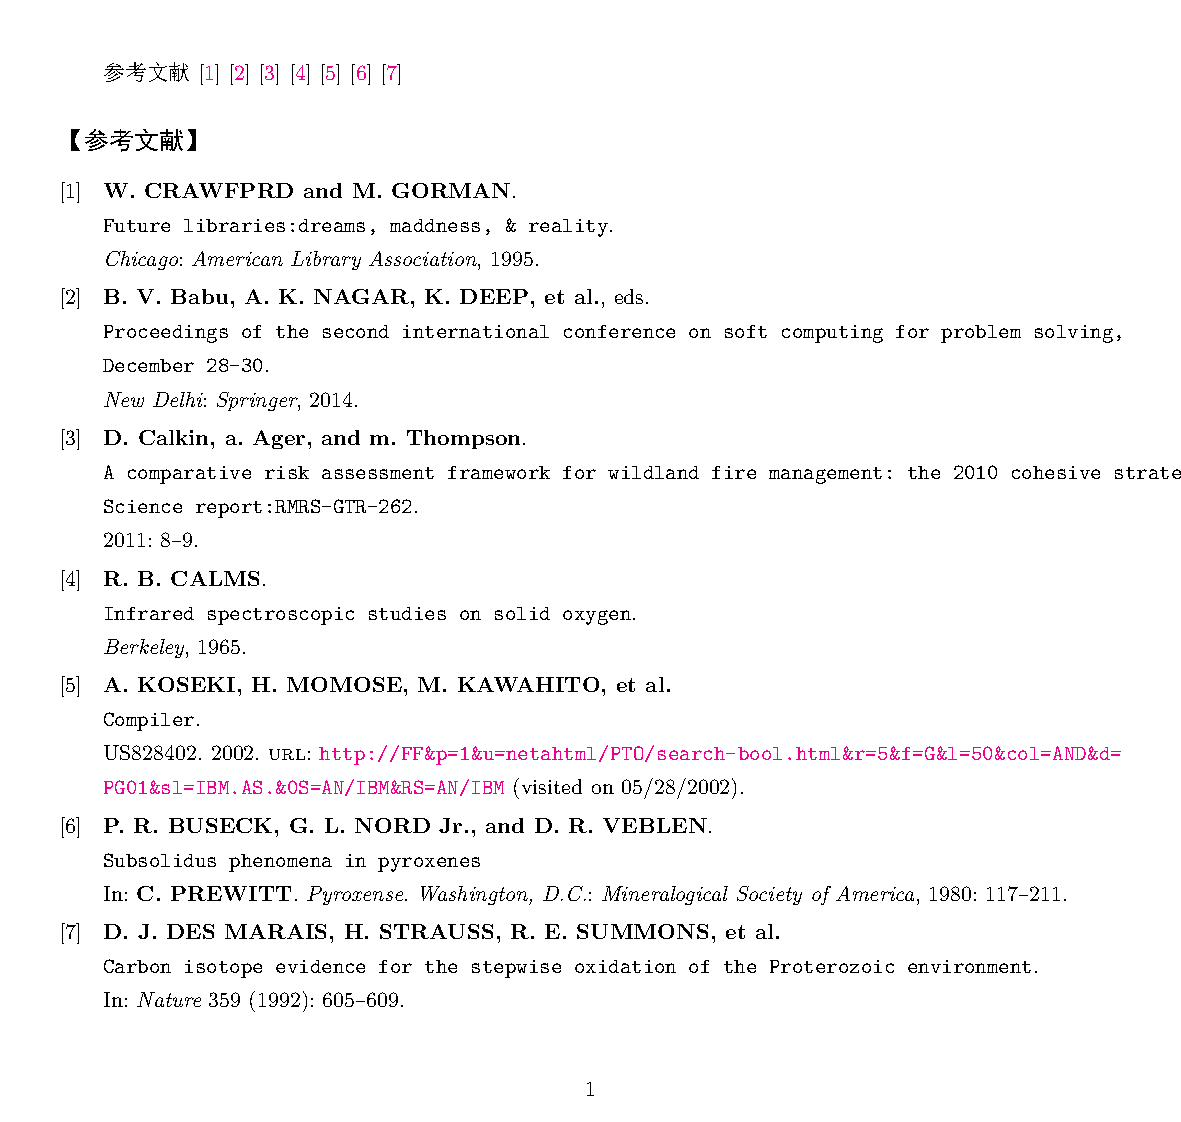
\includegraphics[width=0.8\textwidth,page=1]{egstylecustomize.pdf}}
  \caption{参考文献样式快速定制}\label{bib:style}
\end{figure}

\begin{codetex}{参考文献样式定制举例}{bib:style:customize}
\ProvidesFile{studf.bbx}[2016/12/07 v1.0e biblatex bibliography style]
略,详见源文件。
\end{codetex}
源代码见\href{run:./exampleandimage/studf.bbx}{tex文件}。

如果对于中文参考文献需要一些特殊的处置,那么可以基于gb7714-2015进行修改,如例\ref{style:customize:gb}给出的代码。其结果如图\ref{bib:style:gba},\ref{bib:style:gbb}所示。
\begin{figure}[!htb]
  \centering
  \fbox{
\includegraphics[width=0.7\textwidth,page=1]{egstylecustomizegb.pdf}}
  \caption{国标风格的参考文献样式快速定制A}\label{bib:style:gba}
\end{figure}

\begin{figure}[!htb]
  \centering
  \fbox{
\includegraphics[width=0.7\textwidth,page=2]{egstylecustomizegb.pdf}}
  \caption{国标风格的参考文献样式快速定制B}\label{bib:style:gbb}
\end{figure}

\begin{codetex}{参考文献样式定制举例-国标样式}{style:customize:gb}
\ProvidesFile{gbudf.bbx}[2016/12/07 v1.0e biblatex bibliography style]
略,详见源文件。
\end{codetex}
源代码见\href{run:./exampleandimage/gbudf.bbx}{tex文件}。

\subsection{多语言文献}

不仅GB/T 7714-2015对于多语言文献提出了要求,某些期刊对于参考文献也有双语文献要求,这一问题可以通过条目集类型(set)进行设置,这对于专著和连续出版物的析出文献来说有可能是常用的。设置和使用条目集类型(set)时,有静态和动态两种方法。

\subsubsection{动态方法}
动态方法的使用更方便,直接在写文档时候,将双语文献设置成set,然后引用set的bibtex键。比如:

\begin{codetex}{设置set条目集用于双语文献动态方法}{eg:setforbilangentry}
%file:egbilang.tex
\documentclass{report}
\usepackage{ctex}
\usepackage{geometry}
\geometry{paperwidth=15cm,paperheight=9.5cm,top=0cm, bottom=1.5cm, left=1cm,right=1cm}
\usepackage{titlesec}
\titleformat{\chapter}{\zihao{5}\heiti}{\thechapter}{1em}{}
\titlespacing*{\chapter}{0pt}{0.0\baselineskip}{0.0\baselineskip}[0pt]
\titleformat{\section}{\zihao{-5}\heiti}{\thesection}{1em}{}
\titlespacing*{\section}{0pt}{0.0\baselineskip}{0.0\baselineskip}[0pt]
\usepackage[backend=biber,style=gb7714-2015]{biblatex}
\addbibresource[location=local]{example.bib}

\begin{document}
\chapter{序章}
序章内容\cite{GPS1988--}
\defbibentryset{bilangyi2013}{易仕和2013--,Yi2013--}
\defbibentryset{bilangzhang2007}{张敏莉2007-500-503,Zhang2007-500-503}
专著,双语文献引用\cite{bilangyi2013}\cite{bilangzhang2007}
\printbibliography[heading=subbibliography,title=参考文献]
\end{document}
\end{codetex}

得到的参考文献打印结果如图\ref{bib:eg:bilang}所示。

\begin{figure}[!htb]
  \centering
  \fbox{
\includegraphics[width=\figwd\textwidth,page=1]{egbilang.pdf}}
  \caption{双语文献参考文献}\label{bib:eg:bilang}
\end{figure}

\subsubsection{静态方法}
静态方法是在bib源文件中给出条目集(set)并使用biber后端,条目的域信息采用如下方法定义:
\begin{codetex}{设置set条目集用于双语文献静态方法}{eg:set:static}
@Set{set1,
entryset = {key1,key2,key3},
}
%如果要达到上例动态设置set一样的结果,在bib文件中静态设置set条目如下:
@Set{bilangyi2013,
entryset = {易仕和2013--,Yi2013--},
}
\end{codetex}
当使用bibtex后端时,则需要进一步设置,具体参考biblatex宏包手册。


\subsection{脚注题注小页环境中的引用}

文献不仅仅可以在正文中引用,也可以在脚注,题注,小页环境中引用,下面分别进行说明:

\subsubsection{脚注中的引用}

要在脚注中的引用文献,直接在footnote脚注的内容中添加cite等引用命令即可,比如:

\begin{codetex}{脚注中引用参考文献}{cite:infoot}
%file:egciteinfoot.tex
\documentclass{report}
\usepackage{ctex}
\usepackage{geometry}
\geometry{paperwidth=12cm,paperheight=8cm,top=0cm, bottom=1.5cm, left=1cm,right=1cm}
\usepackage{hyperref}
\usepackage{titlesec}
\titleformat{\chapter}{\zihao{5}\heiti}{\thechapter}{1em}{}
\titlespacing*{\chapter}{0pt}{0.5\baselineskip}{0.5\baselineskip}[0pt]
\titleformat{\section}{\zihao{-5}\heiti}{\thesection}{1em}{}
\titlespacing*{\section}{0pt}{0.5\baselineskip}{0.5\baselineskip}[0pt]
\usepackage[backend=biber,style=gb7714-2015]{biblatex}
\addbibresource[location=local]{example.bib}

\begin{document}
\chapter{序章}
正文内容脚注中引用参考文献\footnote{biblatex使用可以参考宏包手册\cite{Lehman2015}}
\printbibliography[heading=subbibliography,title=本章参考文献]
\end{document}
\end{codetex}

结果如图\ref{fig:eg:citeinfoot}所示。

\begin{figure}[!htb]
  \centering
  \fbox{
\includegraphics[width=\figwd\textwidth,page=1]{egciteinfoot.pdf}}
  \caption{脚注中引用参考文献}\label{fig:eg:citeinfoot}
\end{figure}

\subsubsection{题注中的引用}

在题注中引用文献方法是类似的,直接在caption题注的内容中添加cite等引用命令即可,比如:

\begin{codetex}{题注中引用参考文献}{eg:cite:incaption}
%file:egciteincaption.tex
\documentclass{report}
\usepackage{ctex}
\usepackage{geometry}
\geometry{paperwidth=12cm,paperheight=9cm,top=0cm, bottom=1.5cm, left=1cm,right=1cm}
\usepackage{titlesec}
\titleformat{\chapter}{\zihao{5}\heiti}{\thechapter}{1em}{}
\titlespacing*{\chapter}{0pt}{0.5\baselineskip}{0.5\baselineskip}[0pt]
\titleformat{\section}{\zihao{-5}\heiti}{\thesection}{1em}{}
\titlespacing*{\section}{0pt}{0.5\baselineskip}{0.5\baselineskip}[0pt]
\usepackage{hyperref}
\usepackage[backend=biber,style=gb7714-2015]{biblatex}
\addbibresource[location=local]{example.bib}

\begin{document}
\chapter{序章}
\begin{figure}[!htb]
  \centering
  \fbox{\parbox[c][2cm][c]{4cm}{\centering\large example figure}}
  \caption{在题注中引用文献\cite{GPS1988--}}\label{cite:incaption}
\end{figure}
\printbibliography[heading=subbibliography,title=本章参考文献]
\end{document}
\end{codetex}

结果如图\ref{fig:eg:citeincaption}所示。

\begin{figure}[!htb]
  \centering
  \fbox{
\includegraphics[width=\figwd\textwidth,page=1]{egciteincaption.pdf}}
  \caption{题注中引用参考文献}\label{fig:eg:citeincaption}
\end{figure}

\subsubsection{小页环境中的引用}
在小页环境中引用文献方法是类似的,直接在小页环境的内容中添加cite等引用命令即可,比如:

\begin{codetex}{小页环境中引用参考文献}{eg:cite:inminipage}
%file:egciteinminipage.tex
\documentclass{report}
\usepackage{ctex}
\usepackage{geometry}
\geometry{paperwidth=12cm,paperheight=6cm,top=0cm, bottom=1.5cm, left=1cm,right=1cm}
\usepackage{titlesec}
\titleformat{\chapter}{\zihao{5}\heiti}{\thechapter}{1em}{}
\titlespacing*{\chapter}{0pt}{0.5\baselineskip}{0.5\baselineskip}[0pt]
\titleformat{\section}{\zihao{-5}\heiti}{\thesection}{1em}{}
\titlespacing*{\section}{0pt}{0.5\baselineskip}{0.5\baselineskip}[0pt]
\usepackage{hyperref}
\usepackage[backend=biber,style=gb7714-2015]{biblatex}
\addbibresource[location=local]{example.bib}

\begin{document}
\chapter{序章}
\fbox{
\begin{minipage}{0.5\linewidth}\centering
使用小页环境引用文献\cite{GPS1988--}
\end{minipage}}
\printbibliography[heading=subbibliography,title=本章参考文献]
\end{document}
\end{codetex}

结果如图\ref{fig:eg:citeinminipage}所示。

\begin{figure}[!htb]
  \centering
  \fbox{
\includegraphics[width=\figwd\textwidth,page=1]{egciteinminipage.pdf}}
  \caption{小页环境中引用参考文献}\label{fig:eg:citeinminipage}
\end{figure}


\subsection{脚注旁注中的文献表}

前面说过,biblatex可以访问和利用任何参考文献数据的功能很强大。其中一个功能即将参考文献标放到脚注中,这在某些需要的时候是很有用的。

\subsubsection{使用biblatex命令实现脚注文献表}

biblatex提供了一个footfullcite命令实现将文献表放到脚注中,看例\ref{eg:bib:infoot}给出的代码,3个footfullcite命令将3条文献放入脚注中,文献的著录格式仍然是指定的gb7714-2015ay样式。
\begin{codetex}{脚注参考文献表}{eg:bib:infoot}
%file:egbibinfoot.tex
\documentclass{article}
\usepackage{ctex}
\usepackage[paperwidth=12cm,paperheight=9cm,%
left=1cm,right=1cm,top=1cm,bottom=1.5cm]{geometry}
\usepackage[colorlinks=true,pdfstartview=FitH,linkcolor=blue,
anchorcolor=violet,citecolor=magenta]{hyperref}%书签功能,选项去掉链接红色方框
\usepackage{titleref}%标题引用
\usepackage[backend=biber,style=gb7714-2015ay]{biblatex}
\renewcommand{\bibfont}{\zihao{6}}
\addbibresource[location=local]{example.bib}

\begin{document}
\section{页边的文献表}
参考文献\cite{白书农1998-146-163}
\footfullcite{陈志勇2011--}
\footfullcite{储大同2010-721-724}
\footfullcite{顾炎武1982--}
中文段落参考文献中文段落参考文献中文段落参考文献中文段落参考文献中文段落
参考文献中文段落参考文献中文段落参考文献中文段落参考文献中文段落参考文献
中文段落参考文献中文段落参考文献中文段落参考
\printbibliography[title=【全部引文】]
\end{document}
\end{codetex}

结果如图\ref{fig:eg:bibinfoot}所示。

\begin{figure}[!htb]
  \centering
  \fbox{
\includegraphics[width=\figwd\textwidth,page=1]{egbibinfoot.pdf}}
  \caption{脚注中的参考文献表}\label{fig:eg:bibinfoot}
\end{figure}


\subsubsection{使用biblatex命令和footmisc实现旁注文献表}

旁注文献表可以在脚注文献表的基础上,利用footmisc宏包实现。footmisc的side选项可以将脚注移到页边中,这样脚注参考文献表就变成了旁注参考文献表。例\ref{eg:bib:inmargin}给出测试代码。

\begin{codetex}{旁注参考文献表}{eg:bib:inmargin}
%file:egbibinmargin.tex
\documentclass{article}
\usepackage{ctex}
\usepackage[includemp,paperwidth=12cm,paperheight=9cm,%
left=1cm,right=1cm,marginparwidth=5cm,top=1cm,bottom=1.5cm]{geometry}
\usepackage[colorlinks=true,pdfstartview=FitH,linkcolor=blue,
anchorcolor=violet,citecolor=magenta]{hyperref}%书签功能,选项去掉链接红色方框
\usepackage{titleref}%标题引用
\usepackage[backend=biber,style=gb7714-2015ay]{biblatex}
\renewcommand{\bibfont}{\zihao{6}}
\addbibresource[location=local]{example.bib}
\usepackage[%
%   bottom,      % Footnotes appear always on bottom. This is necessary
%                % especially when floats are used
%   stable,      % Make footnotes stable in section titles
   perpage,     % Reset on each page
%   %para,       % Place footnotes side by side of in one paragraph.
   side,       % Place footnotes in the margin
%   ragged,      % Use RaggedRight
%   marginal,
%   norule,     % suppress rule above footnotes
%   %hang,
%   multiple,    % rearrange multiple footnotes intelligent in the text.
%   %symbol,     % use symbols instead of numbers
]{footmisc}

\begin{document}

\section{页边的文献表}
参考文献\cite{白书农1998-146-163}
\footfullcite{陈志勇2011--}
\footfullcite{储大同2010-721-724}
\footfullcite{顾炎武1982--}
中文段落参考文献中文段落参考文献中文段落参考文献中文段落参考文献中文段落
参考文献中文段落参考文献中文段落参考文献中文段落参考文献中文段落参考文献
中文段落参考文献中文段落参考文献中文段落参考

\newpage
\newgeometry{left=1cm,right=1cm,top=1cm,bottom=2cm}
\printbibliography[title=【全部引文】]
\end{document}
\end{codetex}

结果如图\ref{fig:eg:bibinmargin}所示。

\begin{figure}[!htb]
  \centering
  \fbox{
\includegraphics[width=\figwd\textwidth,page=1]{egbibinmargin.pdf}}
  \caption{旁注中的参考文献表}\label{fig:eg:bibinmargin}
\end{figure}

\subsubsection{使用自定义方式环境方式实现旁注文献表}

旁注的文献表还可以通过自定义参考环境命令的方式实现,这种方式下可以同时存在脚注和旁注参考文献。例\ref{eg:bib:infootmargin}给出测试代码,这也是参考文献表环境定义的一个例子。需要注意,这里定义的命令中使用了kewword域中的引用关键词信息,这一信息是由gb7714-2015样式文件提供的,所以使用这种方式必须加载gb7714-2015样式。而且这里的命令相对比较简单,可以进一步改进。或者也可以利用biblatex提供的接口使用文献的条目类型驱动,具体可以参考Mixing Programming Interfaces 一节。

\begin{codetex}{另一种脚注和旁注参考文献表}{eg:bib:infootmargin}
%file:egbibinfootmargin
\documentclass[twoside]{article}
\usepackage{ctex}
\usepackage{geometry}
\geometry{includemp,paperwidth=21cm,paperheight=19cm,%
left=1cm,right=1cm,marginparwidth=6cm,top=1cm,bottom=1.5cm}
\usepackage{xcolor}
%书签功能,选项去掉链接红色方框
\usepackage[CJKbookmarks,colorlinks,bookmarksnumbered=true,pdfstartview=FitH,linkcolor=blue]{hyperref}
\usepackage[backend=biber,style=gb7714-2015]{biblatex}
\addbibresource[location=local]{example.bib}

%\newcommand{\itemcmd}[1]{#1\par}
\defbibenvironment{marginref}{\begingroup}
{\endgroup}{\zihao{6}\songti}%\newline\itemcmd
\defbibheading{marginref}{}
\newcommand{\pz}[1]{% 定义 pz 为旁注命令
\marginpar[\flushright\textcolor{blue}{\scriptsize#1}]{\scriptsize#1}}
\newcommand{\pzcite}[1]{%
\cite{#1}
\marginpar[\flushright\textcolor{blue}{{\printbibliography[env=marginref,keyword=#1,heading=marginref]}}]
{\printbibliography[env=marginref,keyword=#1,heading=marginref]}}

\begin{document}
\section{脚注和旁注中的文献表}
参考文献\pzcite{Eggrers--}中文段落参考文献中文段落参考文献中文段
参考文献中文段落参考文献中文段落参考文献中文段落参考文献中文段落
参考文献中文段落参考文献中文段落参考文献中文段落参考文献中文段落
参考文献\pzcite{汤万金2013-09-30--}中文段落参考文献中文段落参考
参考文献\footfullcite{刘裕国2013-01-12--}
\footfullcite{Dublin2012-06-14--}
\footfullcite{王夫之1845--}
中文段落参考文献中文段落参考文献中文段落参考文献中文段落
参考文献中文段落参考文献中文段落参考文献中文段落参考文献中文段落

text text text text text text text text text
\fbox{here is a marginpar}\pz{some note.}
text text text text text text text text text
text text text text text text text text text

参考文献中文段落参考文献中文段落参考文献中文
\fbox{这里是旁注}\pz{中文旁注}
段落参考文献中文段落参考文献中文段落参考文献
中文段落参考文献中文段落参考
\printbibliography[title=【参考文献】]
\end{document}
\end{codetex}

结果如图\ref{fig:eg:bibinfootmargin}所示。

\begin{figure}[!htb]
  \centering
  \fbox{
\includegraphics[width=0.8\textwidth,page=1]{egbibinfootmargin.pdf}}
  \caption{脚注和旁注中参考文献表}\label{fig:eg:bibinfootmargin}
\end{figure}

\subsection{文献表分类筛选打印}

除了前述的分章节打印外参考文献可以分类筛选打印,主要基于printbibliography命令的type,nottype,keyword,notkeyword,category,notcategory,filter选项来实现,其中category和filter是人工定义的。
type,nottype分别表示打印是和不是某种条目类型的文献,keyword,notkeyword分别表示打印keywords域中含有或不含有某一个关键字的文献,category,notcategory分别表示是或不是某一设定的category的文献,filter表示属于某一设定筛选器的文献。注意因为category必须要在导言区设置,其实使用并不方便。例\ref{eg:bib:filter}给出了这些选项的测试,分别利用type和keyword区分了图书等文献,定义了collections和standard两个筛选器用于打印论文集会议录和标准文献,定义了名为reportandthesis的category用于打印学位论文和报告。结果如图\ref{fig:eg:bibfilter}所示。

\begin{codetex}{分类筛选打印参考文献表}{eg:bib:filter}
%file:egbibfilter
\documentclass{article}
\usepackage{ctex,hyperref}
\usepackage{geometry}
\geometry{paperwidth=21cm,paperheight=26cm,%
left=1cm,right=1cm,top=1cm,bottom=1.5cm}
\usepackage[backend=biber,style=gb7714-2015]{biblatex}
\addbibresource{example.bib}
\renewcommand{\bibfont}{\zihao{6}}
\usepackage{titlesec}
%\titleformat{command}[shape]{format}{label}{sep}{before}[after]
\titleformat{\section}{\centering\bfseries}{第\thesection 节}{1em}{}[]
\titlespacing*{\section}{0pt}{0.0\baselineskip}{0.0\baselineskip}[0pt]
\titleformat{\subsection}{\flushleft\bfseries}{\S\,\thesubsection}{1em}{}[]
\titlespacing*{\subsection}{0pt}{0.0\baselineskip}{0.0\baselineskip}[0pt]
\DeclareBibliographyCategory{reportandthesis}
\addtocategory{reportandthesis}{汤万金2013-09-30--,Calkin2011-8-9,吴云芳2003--,CALMS1965--}
\begin{document}
文献\cite{张伯伟2002--}\cite{CRAWFPRD1995--}\cite{陈志勇2011--}\cite{Babu2014--}\cite{汤万金2013-09-30--}
\cite{Calkin2011-8-9}\cite{吴云芳2003--}\cite{CALMS1965--}\cite{张凯军2012-04-05--}\cite{KOSEKI2002--}
\cite{全国广播电视标准化技术委员会2007-1-1}\cite{国家环境保护局科技标准司1996-2-3}
\cite{楼梦麟2011-11-12}\cite{BUSECK1980-117-211}\cite{陈建军2010-93-93}
\cite{DESMARAIS1992-605-609}\cite{张田勤2000--}\cite{萧钰2001--}

\printbibliography[type=book,notkeyword=standard,title=【普通图书】]
\defbibfilter{collections}{%
type=collection
or type=proceedings
or type=incollection
or type=inproceedings
}
\printbibliography[filter=collections,title=【论文集、会议录】]
\defbibfilter{standard}{%
( type=book or type=inbook )
and keyword=standard
}
\printbibliography[filter=standard,title=【标准文献】]
\printbibliography[type=inbook,notkeyword=standard,title=【专著中析出的文献】]
\printbibliography[type=article,notkeyword=news,title=【期刊中析出的文献】]
\printbibliography[type=article,keyword=news,title=【报纸析出的文献】]
\printbibliography[category=reportandthesis,title=【报告和学位论文】]
\printbibliography[notcategory=reportandthesis,title=【非报告和学位论文】]
\end{document}
\end{codetex}

\begin{figure}[!htb]
  \centering
  \fbox{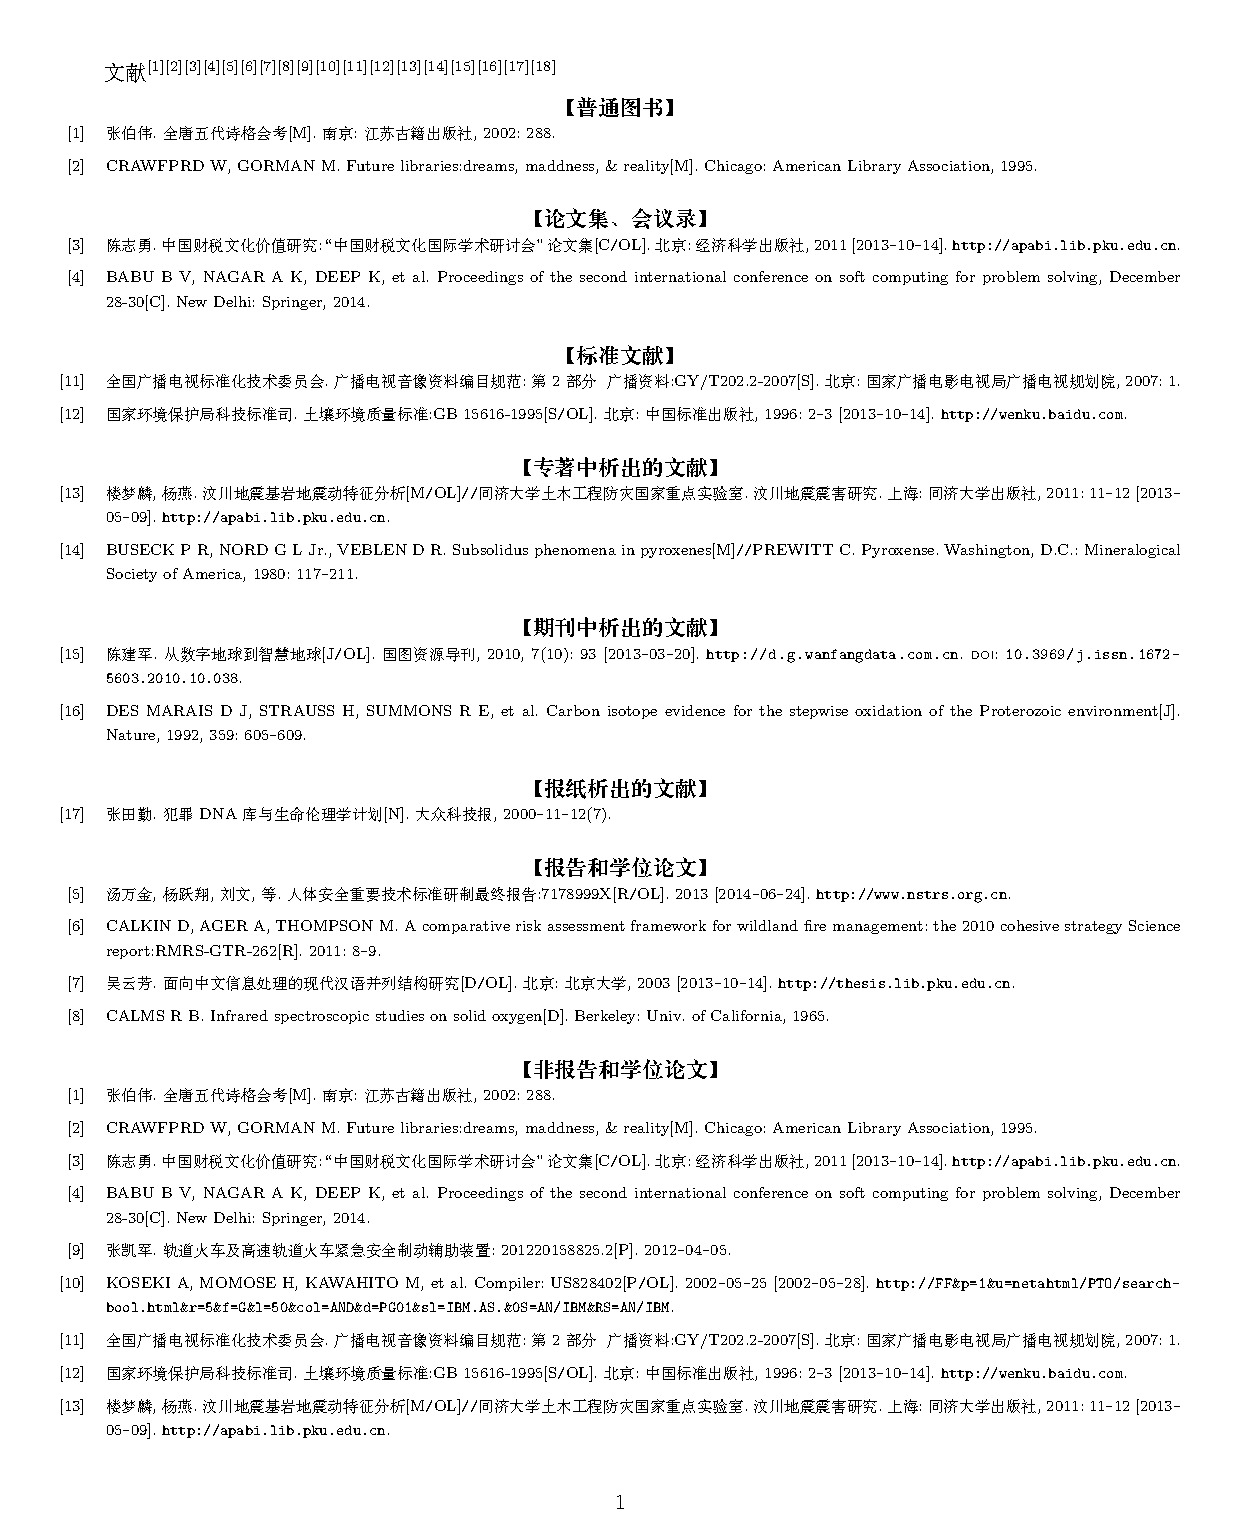
\includegraphics[width=0.8\textwidth,page=1]{egbibfilter.pdf}}
  \caption{脚注和旁注中参考文献表}\label{fig:eg:bibfilter}
\end{figure}

\subsection{beamer类中的参考文献}\label{sec:bib:inbeamer}
在beamer类中使用biblatex生成参考文献与一般文档类中大体上一致,略有差别,主要是refsection无法使用。在实际应用中,beamer 类有两种文献表时主要的,一是文末的文献表,二是脚注中的文献表。

文末的文献表,一般示全局文献,所以可以不使用任何的refsection或者refsegment,也可以使用refsegment环境。不用refsegment时在frame中需要引用的位置加入cite等命令,在某一frame中printbibliography打印处理即可。使用refsegment环境时,将引用参考文献的内容包含在各个refsegment环境中,然后使用一个全局的printbibliography命令遍历各个refsegment并处理并打印。这两种方法在beamer中都可以使用。

脚注中的文献表类似于一般文档类中的做法,使用biblatex提供的footfullcite命令即可。例\ref{eg:bib:beamer}给出了一个测试代码。其结果如图\ref{fig:eg:bibinbeamerfoot},\ref{fig:eg:bibinbeamer}所示。

\begin{codetex}{beamer中使用biblatex参考文献}{eg:bib:beamer}
%file:egbibinbeamer
\documentclass[xcolor=svgnames]{beamer}
\mode<presentation>
\usepackage{ctex}
\usepackage{graphicx}
\usepackage{xcolor}
\usepackage{listings}
\usepackage[backend=biber,style=gb7714-2015]{biblatex}
\renewcommand{\bibfont}{\zihao{8}\songti}
\addbibresource[location=local]{example.bib}

\title{\LaTeX{} 参考文献之 \newline
Biblatex宏包使用和GB/T7714-2015参考文献样式}
%\renewcommand{\thefootnote}{\fnsymbol{footnote}}
\author{胡振震\footnote{hzzmail@163.com}}
\date{\today}
\renewcommand{\footnotesize}{\tiny}

\begin{document}
\begin{frame}[plain]
  \titlepage
\end{frame}

\begin{frame}{测试参考文献}
\tiny
在脚注中引用或者把文献表放到脚注中
\footnote{在脚注中引用\footcite{Saito2006-169-176}}
\footfullcite{中国职工教育研究会1985--}
\footfullcite{Fontana2002-309-313}
\footfullcite{Robertson2011--}
\footfullcite{雷光春2012--}
\footfullcite{Humphrey1971--}
\footfullcite{马欢2011-27-27}
\footfullcite{中国图书馆学会1957--}
\footfullcite{刘彻东1998-38-39}
\end{frame}

\begin{frame}{参考文献}
\printbibliography[heading=bibliography,title=参考文献]
\end{frame}
\end{document}
\end{codetex}

\begin{figure}[!htb]
  \centering
  \fbox{
\includegraphics[width=\figwd\textwidth,page=2]{egbibinbeamer.pdf}}
  \caption{beamer类脚注中的参考文献表}\label{fig:eg:bibinbeamerfoot}
\end{figure}

\begin{figure}[!htb]
  \centering
  \fbox{
\includegraphics[width=\figwd\textwidth,page=3]{egbibinbeamer.pdf}}
  \caption{beamer类全局参考文献表}\label{fig:eg:bibinbeamer}
\end{figure}


\section{结论}
通过本文的工作给出了\LaTeX 文档中文参考文献相关问题的biblatex解决方案包括:基本参考文献生成、分章参考文献、指定格式的著录和标注样式等,基本能够满足日常的各类参考文献生成需求,能够为\LaTeX 文档写作提供帮助。


%%----------------------------------------------------------------
\printbibliography[heading=subbibliography,title=参考文献]
%\end{multicols}
\end{refsection}
\clearpage 
%%一篇论文结束
%%----------------------------------------------------------------


%%================================================================
%%下一篇论文,格式与上一篇类似,只要修改内容即可
%%----------------------------------------------------------------
%新的一篇论文放到articlesecond.tex文件中,后面的新论文类似,通常不包含进来。


%为方便超链接查看,这里可以加入目录
\vspace{1cm}
\noindent\rule{\linewidth}{3pt}
\phantomsection
\addcontentsline{toc}{section}{目录}
\tableofcontents
%\renewcommand{\numberline}[1]{#1~}
\phantomsection
\addcontentsline{toc}{section}{插图}
\listoffigures
\phantomsection
\addcontentsline{toc}{section}{示例}
\listofegcode


\end{document} 